\documentclass{risepaper}
%\卒論
\修論
\usepackage{makeidx}
\usepackage[dvipdfmx]{graphicx}
\usepackage{ascmac}
\usepackage[dvipdfmx]{graphicx}
%\usepackage[dvips]{graphicx}
\usepackage{listings,jlisting}
\usepackage[dvipdfmx]{color}
\usepackage{here}
\usepackage{fancyvrb}
%\usepackage{graphicx}
\renewcommand{\lstlistingname}{ソースコード}
\renewcommand{\lstlistlistingname}{プログラム一覧} 
\lstset{%
  basicstyle={\small},%
  identifierstyle={\small},%
  commentstyle={\small\itshape\color[rgb]{0,0.5,0}},%
  keywordstyle={\small\bfseries\color[rgb]{0,0,1}},%
  ndkeywordstyle={\small},%
  stringstyle={\small\ttfamily\color[rgb]{1,0,1}},
  frame={tb},
  breaklines=true,
  columns=[l]{fullflexible},%
  numbers=left,%
  xrightmargin=0zw,%
  xleftmargin=3zw,%
  numberstyle={\scriptsize},%
  stepnumber=1,
  numbersep=1zw,%
  lineskip=-0.5ex%
}
\usepackage{multirow}
\usepackage{ascmac}
\usepackage{fancybox}
  \title {Blocklyを用いた非手続き型言語のためのプログラミング環境の構築}         
   \author{佐野 裕也}   
   \year{令和元年度~(2019年度)}
   \teacher{香川~考司} 
   \chief{香川~考司}
	\seconda{最所~圭三}
	\secondb{高木~智彦}
	\date{令和2年2月8日}                       
% \date{\today}
                                                          
\makeindex                                                
                                         
%\etitle{Development of programming learning support environment for\\ multilingual support using Blockly}
% 2006/2/7改訂
% タイトルを複数行にしたいときは、下のetitleenv環境を使ってください。
\begin{etitleenv}
Construction of a Learning Environment for Multiple Programming Languages using Blockly
\end{etitleenv}

\begin{eabstract}
When a learner studies his second or third programming language, he has to learn its basic concepts and its grammar at the same time in a short period, which is a heavy burden for him. We adopt Blockly, a library for constructing a block-type programming environment for beginners, and try to build a programming learning environment for languages other than procedural ones by using Blockly’s dynamic transformation behavior of blocks. Supported languages are C, JavaScript, Haskell, Bison Flex, Prolog, Scheme, and Python. In each language system, several new blocks corresponding to the grammar corresponding to the programming language are implemented, and in order to maintain the flexibility of the programming language, the function of dynamically transforming the blocks is also extended. At this time, the operation of the system needs to be easy because the purpose is to reduce the burden on the programming learner. Therefore, we will create a tutorial page that specifies the functions of the system and how to assemble the blocks. With these implementations, it is possible to build an environment that makes it easy for beginners to learn basic programming concepts, corresponding to the programming languages learned in university classes.

\end{eabstract}

\begin{jabstract}
学習者は、第2、第3のプログラミング言語を勉強するとき、その基本概念とその文法を短時間で同時に学習する必要があり、これは学習者にとって大きな負担になる。 この問題を解決するために本研究では、初心者向けのブロック型プログラミング環境を構築するためのライブラリであるBlocklyを採用し、Blocklyのブロックの動的変換機能を利用して、手続き言語以外の言語向けのプログラミング学習環境の構築を試みる。対応言語は、C、JavaScript、Haskell、Bison Flex、Prolog、Scheme、Python である。それぞれの言語システムでプログラミング言語に対応した文法に対応した新たなブロックをいくつか実装し、プログラミング言語の柔軟性を保持するために、ブロックの動的変形機能の拡張も行う。その際に、プログラミング学習者の負担を軽減させることが目的なので、システムの操作は容易である必要がある。そこで、システムの各機能の説明、ブロックの組み立て方などを明記したチュートリアルのページを作成する。これらの実装により、大学の授業で学ぶプログラミング言語に対応して、プログラミング初学者がプログラミングの基礎概念を学習しやすい環境を構築できるようにする。

\end{jabstract}


\begin{keyword}
プログラミング学習, ビジュアルプログラミング, C, JavaScript, Haskell, Flex, Prolog, Scheme, Python, Webベース
\end{keyword}

\begin{document} 
\maketitle
%  \listoffigures % 図の目次
%  \listoftables  % 表の目次
                                                          
   \chapter{はじめに}
   
   \section{はじめに}


  プログラミング学習者は、以下の2つを同時に学ばなければならない。
  
\begin{itemize}
\item プログラミングの基礎概念
\item 各プログラミング言語の文法
\end{itemize} 

 これらを学ぶことは、学習者にとって大きな負担である。この負担を軽減するために、ビジュアルプログラミング環境を利用して学習するという選択肢がある。ビジュアルプログラミング環境とは、プログラムをテキストで記述するのではなく、視覚的なオブジェクトでプログラミングするプログラミング環境である。代表的なビジュアルプログラミング環境に、Scratch\cite{Scratch}やWaterbear\cite{waterbear}などがある。本研究では、ビジュアルプログラミング環境を構築するためのJavaScriptライブラリであるBlockly\cite{Blockly}を用いる。
  
Blockly は、Google によって開発された。ブロックを繋ぎ合せることでプログラミングを行う。Blockly を利用することで構文エラーに悩まされず、直感的にプログラミングをすることができる。JavaScript で記述されており、ドキュメントも豊富に用意されているためカスタマイズが容易である。また、Blockly で作成されるプログラムはWeb ベースのアプリケーションであるため、導入の作業が不要である。さらに、Blocklyアプリケーションで作成したブロックは、ライブラリにもともと備わっている機能で、JavaScript、Dart、Python、Lua、PHP の5種類のコードに変換して出力することができる。

   \section{Webベースの利点}
   
本研究で開発したシステムは、Webベースシステムである。Webベースにすることにより、学習者に次のような利点があると考えられる。

\begin{itemize}
\item システムのインストールが不要である
\item Webブラウザがあれば実現可能である
\item 常に最新版のシステムが利用可能である
\end{itemize} 

また、教員側にも次のような利点がある。

\begin{itemize}
\item システムのカスタマイズが容易である
\item システムの不具合をすぐに修正可能である
\item 導入に関する指導が不要である
\end{itemize} 
 
     \section{目的}

本大学・大学院の授業で学習するプログラミング言語には、C、Java、JavaScript、PHP、Haskell、Flexなどがあるが、いずれの言語もそれぞれの特性を持っており、その特性を踏まえて何も無い状態からソースコードを記述するまで理解するにはかなりの時間と負担がかかる。前の項でも述べた通り、Blocklyはプログラミング入門者に適したシステムなのだが、大学の授業で学習するプログラミング言語に一部対応していない。

これらの問題点を踏まえて、Blockly を用いて、さまざまなプログラミング言語に対応したシステムを構築することが必要である。
例えば、関数型言語のHaskellはパターンマッチングを行うが、既存のBlocklyにある関数定義ブロックではこのパターンマッチングに対応しておらず、新たに定義する必要がある。このように、プログラミング言語の文法の違いで新たにブロックを定義する必要がある。また、柔軟性のあるプログラミング言語をブロックの形状によって制約されてしまう。プログラミング言語の柔軟性を保持するために、ブロックの動的変形機能を拡張する。
その際に、プログラミング学習者の負担を軽減させることが目的なので、システムの操作は容易である必要がある。

本論文では、第2章でBlocklyについて、第3章で実装したシステム、第4章でシステムの評価、第5章でまとめ、今後の課題について述べる。
 	
 	\section{関連技術}
    
初学者のプログラミングを学習するためのあらゆる負担を少なくするため、多くのブロックベースのプログラミング学習環境が開発されている.ここではその一部を紹介する。

    \subsection{Scratch}
 
Scratch\cite{Scratch} は MIT メディアラボが開発したブロックベースのプログラミング学習環境である。8 歳から 16 歳向けに設計されており、150 以上の国と地域で利用され、40 以上の言語に対応している。初心者が最初に正しい構文の書き方を覚えること無く結果を得られる、遊び心のある実験やインタラクティブアニメーション、ゲームなどの製作を通してさらなる学習のやる気を起こさせることを意図している。Scratch のイメージを図\ref{fig:scratch}に示す。 

\begin{figure}[h]
\begin{center}
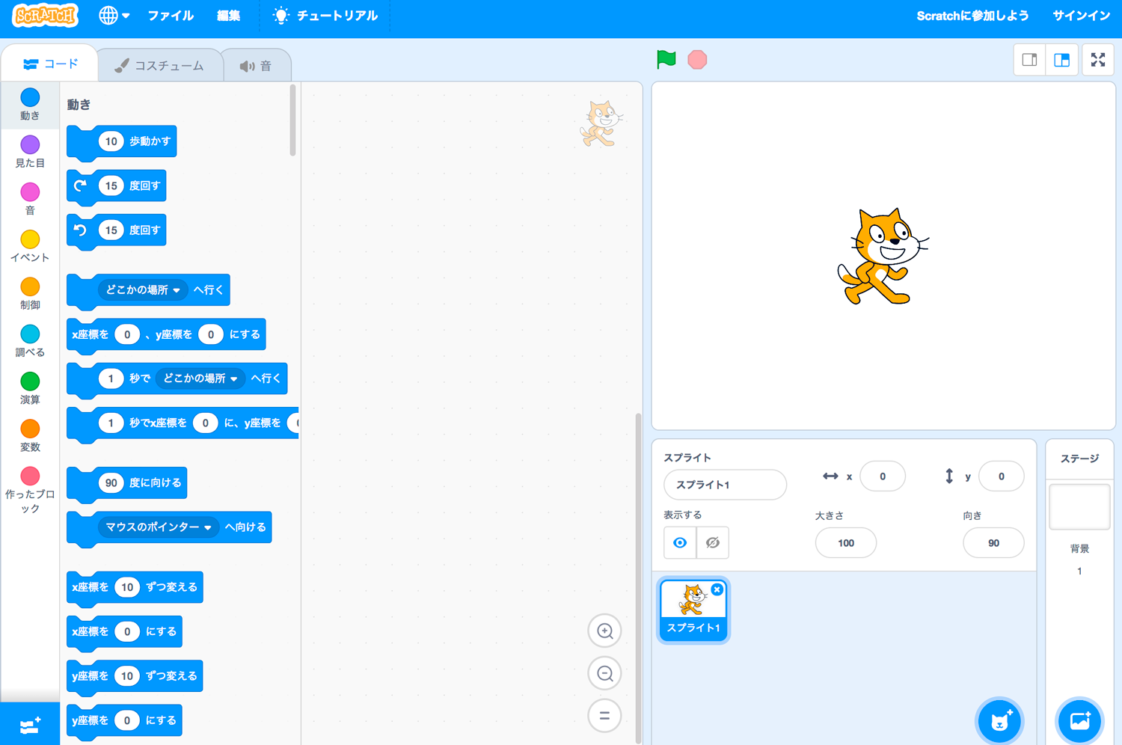
\includegraphics[scale=0.3]{img/scratch.png}
\caption{Scratchのイメージ}%
\label{fig:scratch}
\end{center}%
\end{figure}% 

	\subsection{Waterbear}
    
Waterbear\cite{waterbear}は、2011年5月2日から3日にポートランドで開催されたJSConfで発表したDethe Elzaの発案によるものである。Waterbearの由来は、このシステムが世界中の極端な環境で見られる顕微鏡動物のように、非常に堅牢な言語にしたいからである。Waterbear のイメージを図\ref{fig:waterbear}に示す。 

\begin{figure}[h]
\begin{center}
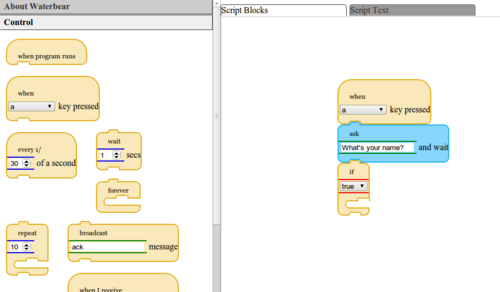
\includegraphics[scale=0.5]{img/waterbear.png}
\caption{Waterbearのイメージ}%
\label{fig:waterbear}
\end{center}%
\end{figure}% 

	\subsection{Snap!}

Snap! は、無料のブロックベースの教育用グラフィカルプログラミング言語およびオンラインコミュニティである。数学や計算の思考を学びながら、インタラクティブなアニメーション、ゲーム、ストーリーなどを探索、作成、編集することを目的としている。Scratchから影響を受けていて、Snap! には多くの高度な機能がある。Snap! のイメージを図\ref{fig:snap}に示す。 

\begin{figure}[h]
\begin{center}
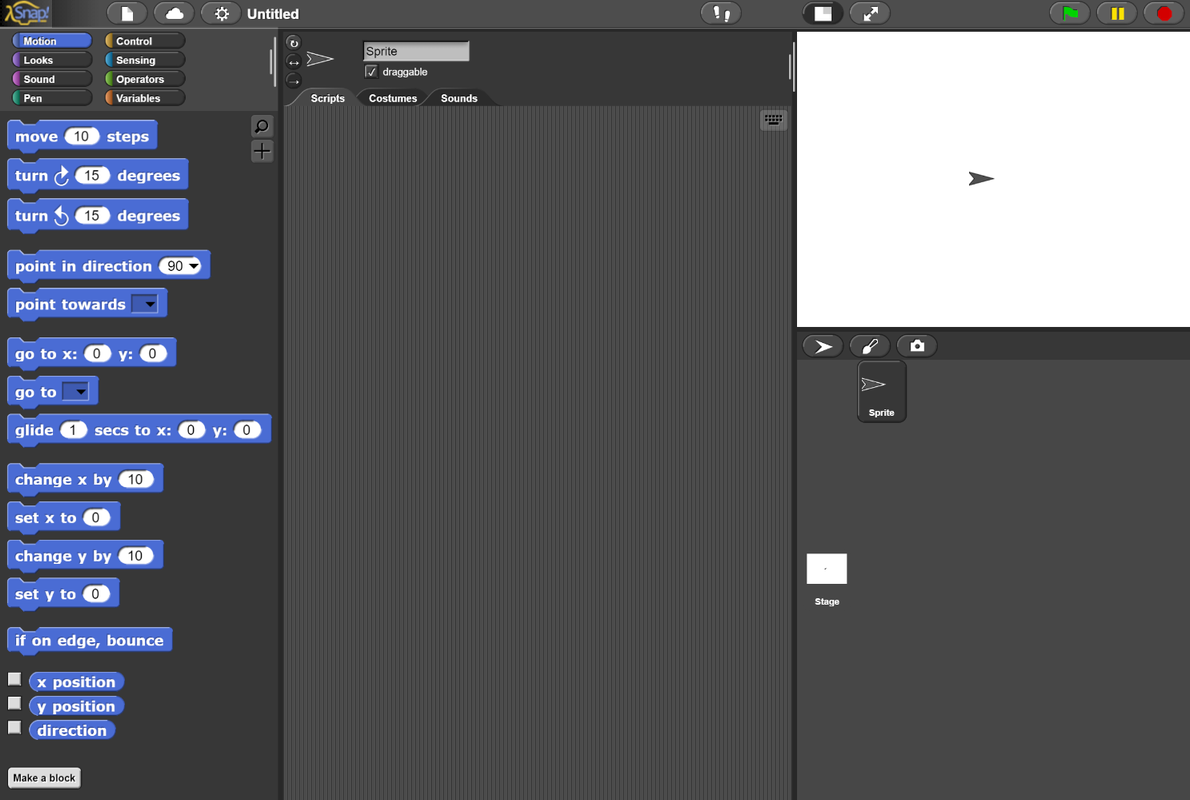
\includegraphics[scale=0.5]{img/snap.png}
\caption{Snap!のイメージ}%
\label{fig:snap}
\end{center}%
\end{figure}% 

    \section{関連研究}
    
    \subsection{Webベースグラフィカルプログラミングエディターを用いた円滑な移行が可能なC言語学習支援環境の開発}
 
 本大学の2014年度の尾崎による修士論文\cite{ozaki}の研究である。
 尾崎の研究は、BlocklyをC言語、Flex言語に適用したもので、システムの対象者はプログラミング入門者である。このシステムによって文法を意識せずにプログラミンングを学ぶことができる。しかし、大学の講義で学習する言語のすべてに対応していない。システム自体が便利であっても、対応していない言語に対しては、このシステムを利用することができない。また、ブロックの形を動的に変形することができないため、柔軟性のあるプログラミング言語をブロックの形状によって制約されてしまうことになる。尾崎の研究で実装したシステムのイメージを図\ref{fig:ozaki}に示す。 


\begin{figure}[h]
\begin{center}
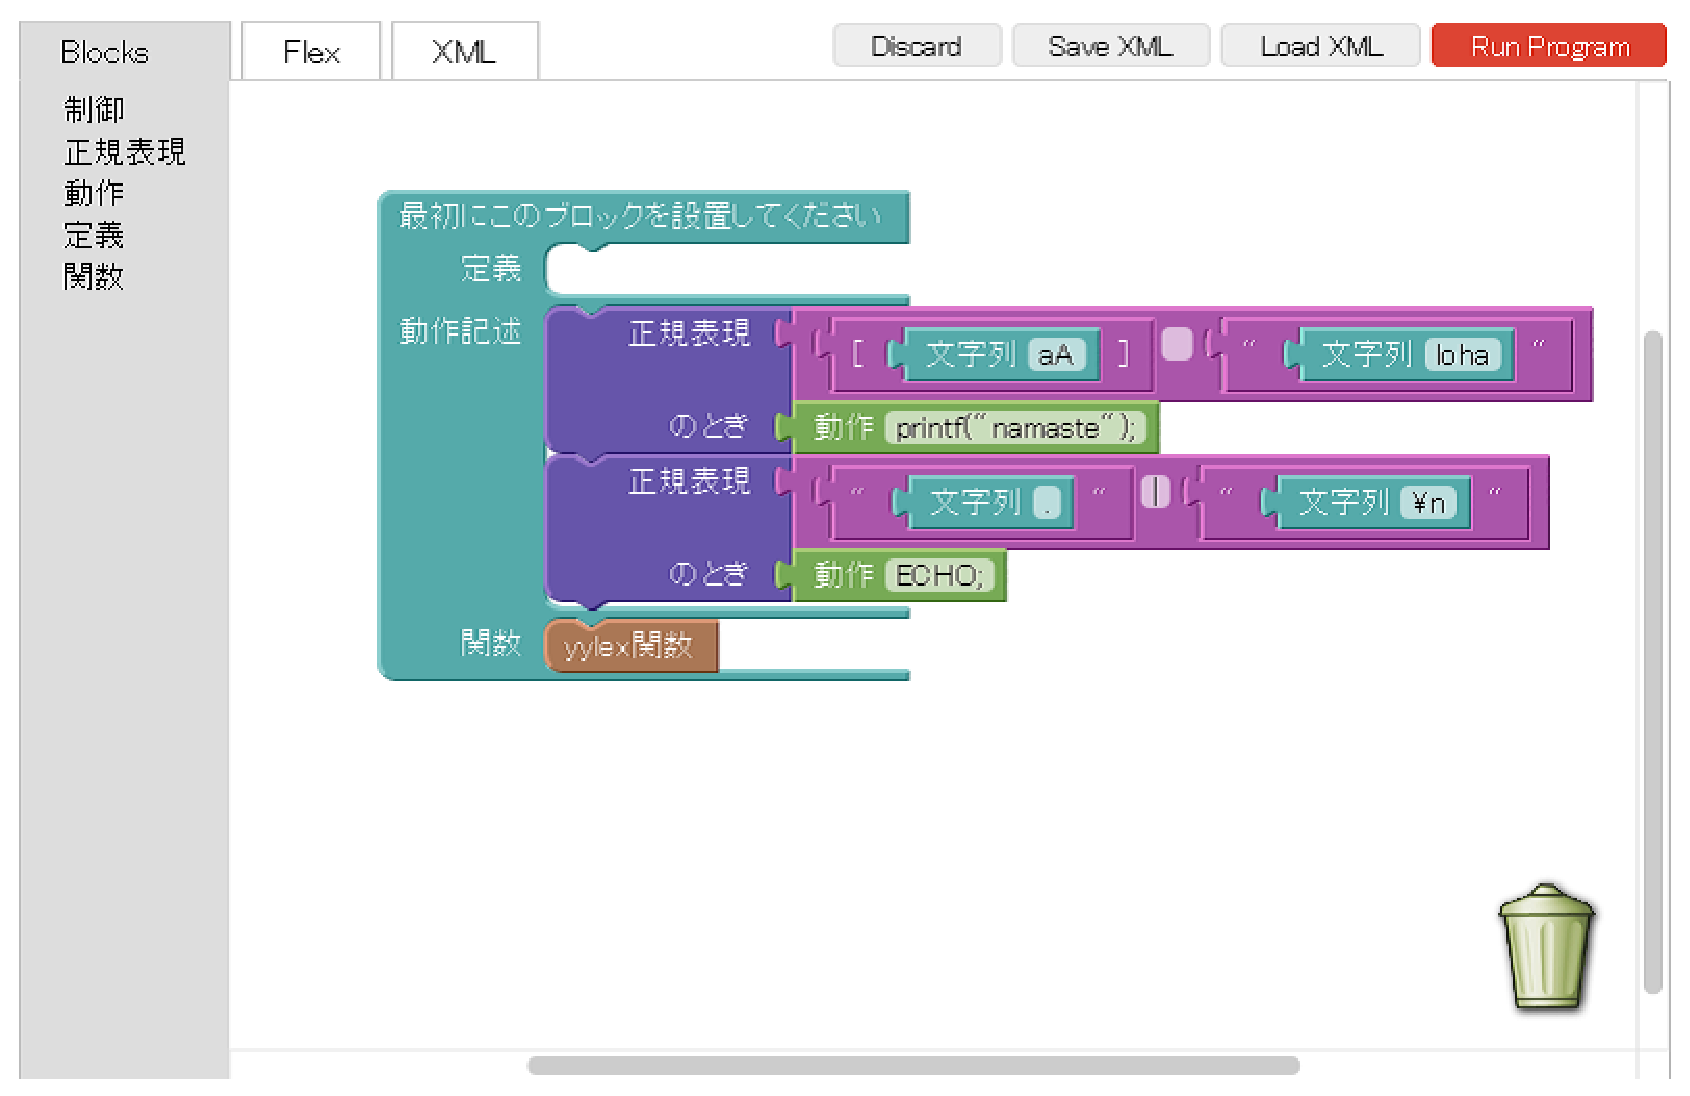
\includegraphics[scale=0.5]{img/ozaki.eps}
\caption{尾崎の研究で実装したシステム}%
\label{fig:ozaki}
\end{center}%
\end{figure}% 
 
	\subsection{Blockly プログラム生成の自動化によるWebベースC言語学習支援環境の機能拡張}
 
  本大学の山形による2017年度の修士論文\cite{yamagata}\cite{yamagata2}である。
 山形は、汎用的なブロックの作成と、Haskell によるパーサーを用いてC 言語のソースコードからBlocklyのブロック定義とBlockly のプログラムに対応するXML 作成の自動化を行い、Blockly を用いたC 言語学習支援環境に追加することで機能を拡張した。Blockly 用のXML をソースコードから簡単に変換することが出来るため、指導者が初学者に提示する練習問題の作成をスムーズに行える。また、プログラミング初学者がBlockly を用いたC 言語学習支援環境を使用しC 言語の予習を行うだけでなく、ブロックベースからテキストベースに移行後はXML の自動生成を利用して学習者が作成したソースコードをXML に変換しBlockly のブロックとして確認することで、理解度の確認に使用することが可能となる。本研究では、C言語以外のソースコードでもブロックを生成できるか検討する。山形の研究で実装したシステムのイメージを図\ref{fig:yamagata}に示す。 
 
\begin{figure}[h]
\begin{center}
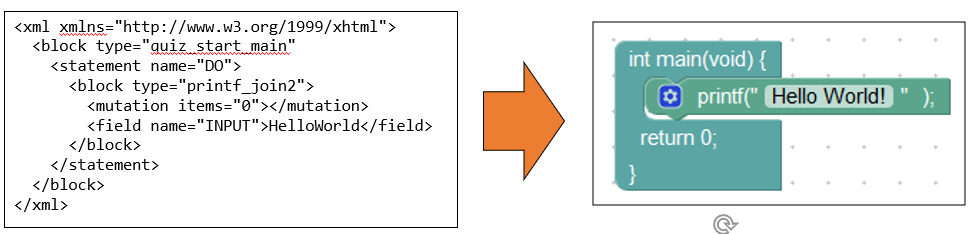
\includegraphics[scale=0.8]{img/yamagata.PNG}
\caption{山形の研究で実装したシステム}%
\label{fig:yamagata}
\end{center}%
\end{figure}% 

	\subsection{Blockly をベースとしたOCamlビジュアルプログラミングエディタ}
    
こちらは、お茶の水女子大学の論文\cite{otya}で、著者は、松本晴香、浅井健一である。
松本らの研究では、Google の提供するビジュアルプログラミングツールBlockly をベースとして、型システムや変数束縛を直感的なユーザインタフェースとして備えたOCamlエディタOCaml Blockly を実装した。Blockly の直感的なプログラム体験を維持しつつ、不正なプログラムを構成することを制限したユーザインタフェースを提案する。let 多相を含む型システムを実装し、結果の型や型変数を形や色として出力し、変数束縛やスコープ範囲を視覚的に表現した。関数型言語であるOcamlをBlocklyに適用された点を参考にしながら、本研究ではHaskell言語をBlocklyに対応させることを目指す。松本らの研究で実装したシステムのイメージを図\ref{fig:otya}に示す。 

\begin{figure}[h]
\begin{center}
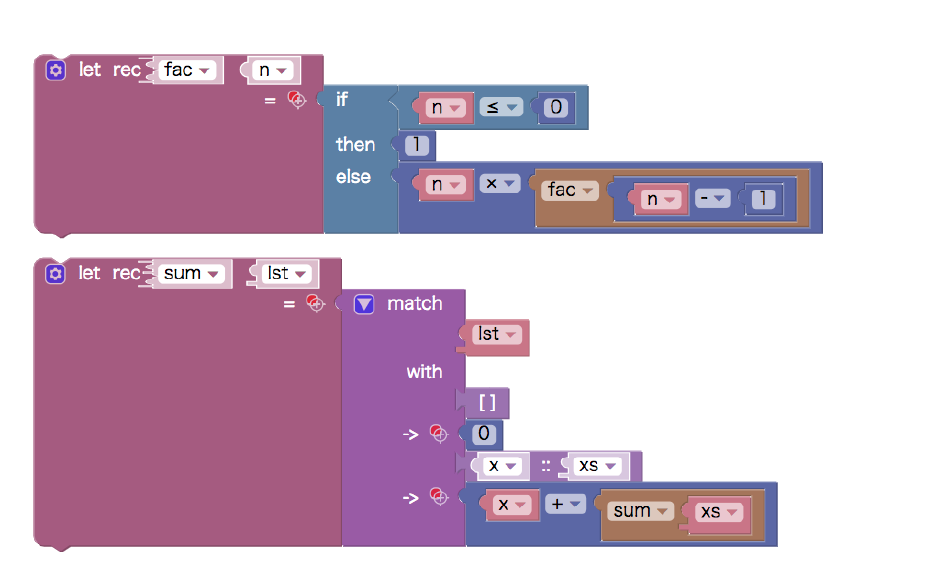
\includegraphics[scale=0.8]{img/otya.PNG}
\caption{松本らの研究で実装したシステム}%
\label{fig:otya}
\end{center}%
\end{figure}% 

	\subsection{To Block or not to Block, That is the Question: Students’ Perceptions of Blocks-based Programming}
    
こちらは、国際学会 IDC'15で発表された論文\cite{idc}で、著者はアメリカ合衆国ノースウェスタン大学所属の David Weintrop と Uri Wilensky である。
David Weintroprらの研究では、高校生がブロックベースのプログラミングツールをどのように見ているか、そのツールの使いやすさに貢献しているもの、ブロックベースのプログラミングとテキストベースのプログラミングの違いが最も顕著なものを調査した結果を報告している。高校生は、ブロックの自然言語記述、ドラッグアンドドロップ構成のやりとり、言語のブラウジングの容易さなど、ブロックベースのプログラミングを容易にするために、多くの要素が役立っていると報告している。また、高校生は、従来のテキストベースのアプローチと比較して、信頼性の欠如やブロックベースのプログラミングの欠点も特定している。この研究での発見は、ブロックベースのプログラミングとテキストベースのプログラミングとの間の識別された違いとともに、公立高校の環境でこのようなツールを使用することの適切性を理解するのに役立ち、そして既存のプログラミングツールの新機能や改訂版の設計に役立つことができる。

\begin{figure}[h]
\begin{center}
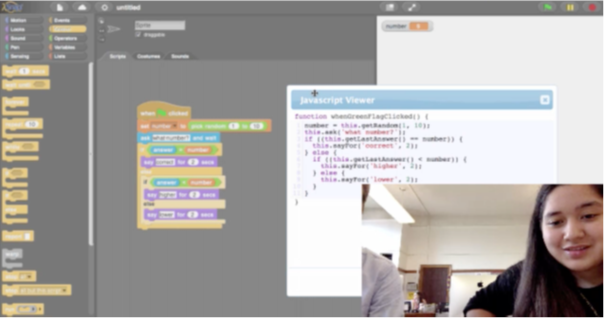
\includegraphics[scale=0.8]{img/idc.png}
\caption{高校生へのインタビューの様子}%
\label{fig:idc}
\end{center}%
\end{figure}% 

   \chapter{Blockly}
  
  
   \section{システム構成}
   
典型的なBlocklyアプリケーションは、ワークスペース部、ブロックメニュー部、ソースコード部、XMLコード部の4つのコンポーネントによって構成される。図\ref{fig:Blockly}にBlocklyアプリケーションのイメージを示す。デフォルトでは、ワークスペース部が表示されており、ソースコードタブを押すとソースコード部のコンポーネントに切り替わり、XMLコードタブを押すとXMLコード部のコンポーネントに切り替わる。ブロックメニュー部は常に左部に表示されている。ここでは、それぞれのコンポーネントについて説明する。
  

\begin{figure}[h]
\begin{center}
\includegraphics[scale=0.4]{img/Blockly.eps}
\caption{Blockly}%
\label{fig:Blockly}
\end{center}%
\end{figure}% 

   \subsection{ワークスペース部}

ワークスペース部は、ブロックを使ってプログラミングを行うスペースである。図\ref{fig:workspace}にワークスペース部のイメージを示す。ユーザは、ブロック部に存在するブロックをワークスペース部にドラッグ&ドロップで自由につなぎ合わせることでプログラミングを行う。ワークスペース部の右下にはゴミ箱アイコンが存在する。ワークスペース部に設置したブロックをこのアイコンにドラッグすると、ブロックを削除することができる。その上に拡大縮小アイコン、さらにその上に中央に寄せるアイコンが表示されている。

また、ワークスペース部に設置したブロックを右クリックすることで、以下のような動作が行える。

\begin{itemize}
\item ブロックの複製
\item コメントの追加
\item ブロックの接続表現の切り替え
\item ブロックの表現の簡略化
\item ブロックの透明化
\item ブロックの削除
\item ブロックの動作を説明するWebページの表示
\end{itemize} 
   
\begin{figure}[h]
\begin{center}
\includegraphics[scale=0.3]{img/workspace.eps}
\caption{ワークスペース部}%
\label{fig:workspace}
\end{center}%
\end{figure}% 

   \subsection{ブロックメニュー部}
   
ブロックメニュー部は、定義されたブロックが存在するスペースである。図\ref{fig:blockmenu}にブロックメニュー部のイメージを示す。ブロックは、論理、数、リストなどのカテゴリーにそれぞれ格納され、カテゴリーをクリックすると、そのカテゴリーに格納されたブロックが表示される。図\ref{fig:blockmenu_open}にカテゴリーをクリックしたときのイメージを示す。ユーザは、このブロックメニューから新たに必要なブロックを選択して使用する。

\begin{figure}[h]
\begin{center}
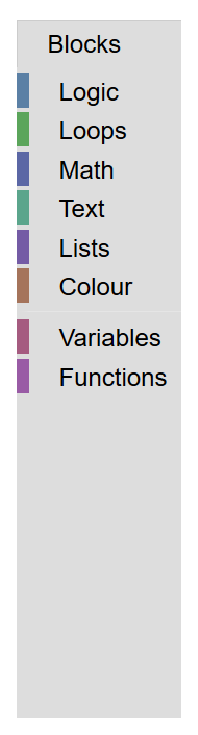
\includegraphics[scale=0.3]{img/blockmenu.eps}
\caption{ブロックメニュー部}%
\label{fig:blockmenu}
\end{center}%
\end{figure}% 

\begin{figure}[h]
\begin{center}
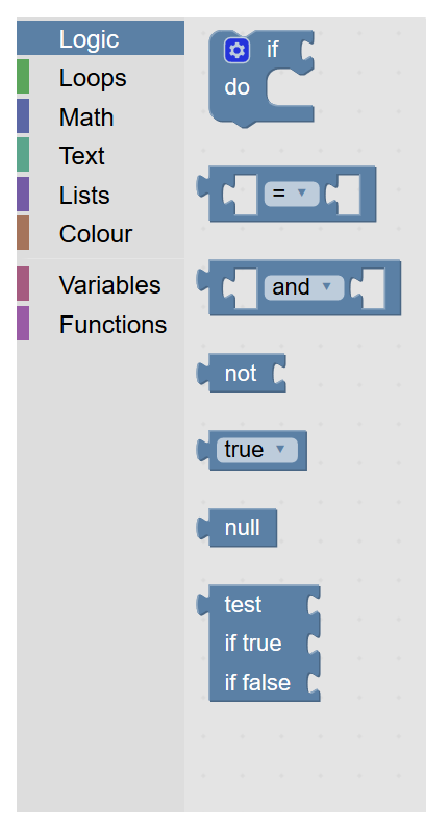
\includegraphics[scale=0.3]{img/blockmenu_open.eps}
\caption{カテゴリーをクリックしたとき}%
\label{fig:blockmenu_open}
\end{center}%
\end{figure}% 

   \subsection{ソースコード部}
   
ソースコード部は、作成したプログラムのソースコードを表示するスペースである。図\ref{fig:source_code}にソースコード部のイメージを示す。タブ名は各プログラミング言語の名称になる。ワークスペース部でブロックを組み合わせて作成したプログラムが、ソースコードに変換され、このソースコード部でいつでも確認することができる。この機能によって、Blocklyでプログラミングを学んだ学習者がソースコードを記述できるように支援する働きを持つ。システムの拡張の際に新たなブロックを実装した場合は、新たなブロックの定義と共に新たにソースコードも定義しなければならない。

\begin{figure}[h]
\begin{center}

\includegraphics[scale=0.5]{img/source_code.eps}
\caption{ソースコード部}%
\label{fig:source_code}
\end{center}%
\end{figure}% 

   \subsection{XMLコード部}
   
XMLコード部は、作成したブロックに対応するXMLコードを表示するスペースである。図\ref{fig:XML_code}にXMLコード部のイメージを示す。ワークスペースで組み合わせたブロックの構造がXML形式で出力され、その出力されたXMLコードをセーブ、ロードすることができる。この機能によって、組み合わせたブロックを保存したり、他の学習者や教員が組み合わせたブロックを自分のワークスペース上に再現することができる。以下は、Blocly for C におけるもしも実行ブロックのXMLコードである。blockという要素タグに、type、id、x、y の4つの属性がある。typeの属性値には、ブロックの名前が入り、idの属性値は20文字のランダムな文字列が入り、idは重複しないようになっている。x、y の属性値はワークスペース上の座標が入る。

\shadowbox{
\begin{minipage}[t]{15cm}
\begin{verbatim}
<block type="controls_if" id="RllK?egbl/90CZu2p_wZ" x="-2" y="27"></block>
\end{verbatim}
\end{minipage}
}



\begin{figure}[h]
\begin{center}
\includegraphics[scale=0.3]{img/XML_code.eps}
\caption{XMLコード部}%
\label{fig:XML_code}
\end{center}%
\end{figure}% 

   \section{Mutator機能}
   
Blocklyの機能にMutatorがある。Mutatorは、ブロックの動的変形を行い、その結果を XML に保存する機能、およびXMLからロードする機能である。図\ref{fig:mutator1}にMutatorのイメージを示す。Mutatorの機能が使えるブロックには、左上に歯車がある場合がある。その歯車のマークを押すと、その近くに吹き出しの形をした小窓が現れる。小窓の左半分はブロックメニュー部、右半分はワークスペース部となっている。小窓の中のコンポーネントは、このブロック限定のものである。小窓のブロックメニュー部から拡張したいブロックを取り出し、小窓のワークスペース部の既存のブロックに取り付ける。すると、吹き出し元のブロックが変形される。図\ref{fig:mutator2}が、そのときのイメージである。Mutator機能によって、ブロックの形をカスタマイズでき、ブロックメニュー部で用意されるブロックの種類を大幅に減らすことができる。

\begin{figure}[h]
\begin{center}
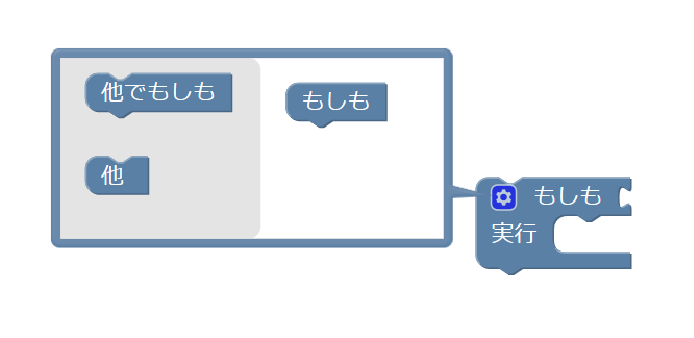
\includegraphics[scale=0.5]{img/mutator1.eps}
\caption{動的変形前のMutatorブロック}%
\label{fig:mutator1}
\end{center}%
\end{figure}% 

\begin{figure}[h]
\begin{center}
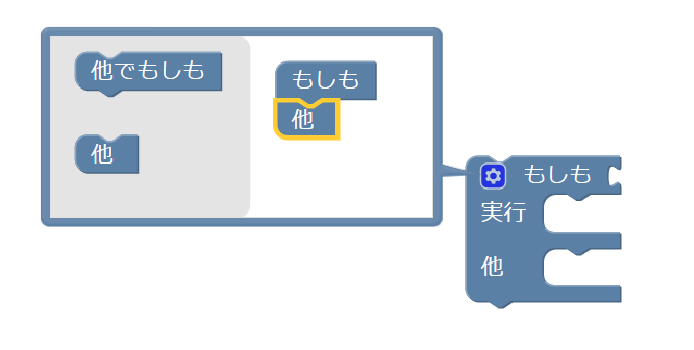
\includegraphics[scale=0.5]{img/mutator2.eps}
\caption{動的変形後のMutatorブロック}%
\label{fig:mutator2}
\end{center}%
\end{figure}% 

   \section{ブロックの定義}
   
ここで、ブロックの定義方法について述べる。
まず初めに、一般的なブロック定義のソースコードを以下に示す。
ブロックの形状を定義したいときは、init関数のなかに関数を記述していく。

\begin{lstlisting}[basicstyle=\ttfamily\footnotesize]
Blockly.Blocks['sample_name'] = {
  init: function() {
    this.setColour(100);
    this.appendDummyInput().appendField("サンプル");
    this.setPreviousStatement(true);
    this.setNextStatement(true);
    this.setOutput(true, 'String');
    this.appendValueInput('A');
    this.setInputsInline(true);
    this.appendStatementInput('DO0');
    this.setTooltip("このブロックは、サンプルです。");
  }
};
\end{lstlisting}

Blocklyには新たなブロックを定義するためにいくつかの関数が用意されている。以下にそれぞれの関数の機能と使用方法を示す。

\begin{itemize}

\item appendField

appendFieldは、ブロック上に文字列や入力フォーム、ドロップダウンメニューを定義する関数である。この関数の前にappendDummyInput関数などを呼び出す必要がある。
以下は、appendFieldの使用例である。

\shadowbox{
\begin{minipage}[t]{14cm}
\begin{verbatim}
this.appendDummyInput().appendField("サンプル");
\end{verbatim}
\end{minipage}
}

\item setColor

setColorは、ブロックの色を定義する関数である。0から360までにの数値を指定することで、ブロックの色を定義することができる。
以下は、setColorの使用例である。

\shadowbox{
\begin{minipage}[t]{14cm}
\begin{verbatim}
this.setColour(100);
\end{verbatim}
\end{minipage}
}

\item setPreviousStatement

setPreviousStatementは、ブロック上接続部の有無を定義する関数である。第1引数がtrueなら接続部が有りで、falseなら無しである。
以下は、setPreviousStatementの使用例である。

\shadowbox{
\begin{minipage}[t]{14cm}
\begin{verbatim}
this.setPreviousStatement(true);
\end{verbatim}
\end{minipage}
}

\item setNextStatement

setNextStatementは、ブロック下接続部の有無を定義する関数である。この関数も同様に、第1引数がtrueなら接続部が有りで、falseなら無しである。
以下は、setNextStatementの使用例である。

\shadowbox{
\begin{minipage}[t]{14cm}
\begin{verbatim}
this.setNextStatement(true);
\end{verbatim}
\end{minipage}
}

\item setOutput

setOutputは、ブロック左接続部の有無を定義する関数である。第1引数がtrueなら接続部が有りで、falseなら無しである。第2引数は、接続先のブロック型を指定する。接続先のブロックの型が指定したものと同じならブロックを接続することができる。型の指定がない場合は、第2引数ごと無くすか、nullを指定する。
以下は、setOutputの使用例である。

\shadowbox{
\begin{minipage}[t]{14cm}
\begin{verbatim}
this.setOutput(true, 'String');
\end{verbatim}
\end{minipage}
}

\item appendValueInput

appendValueInputは、ブロック右接続部の有無を定義する関数である。この接続部に関する関数は、1つのブロックに対し複数指定できる。第1引数には、接続部の名称を指定できる。接続部の名称を指定することで、ブロックの他の接続部と区別させるためである。一般には、変数ブロックや数ブロックを接続する。setCheck関数をそのあとにつけることで接続先のブロックの型を指定できる。
以下は、appendValueInputの使用例である。

\shadowbox{
\begin{minipage}[t]{14cm}
\begin{verbatim}
this.appendValueInput('A').setCheck('int');
\end{verbatim}
\end{minipage}
}

\item setInputsInline

setInputsInlineは、appendValueInput関数で定義した右接続部をブロックの内側にするかを定義する関数である。第1引数がtrueなら内側接続として定義し、falseなら右接続部そのままである。
以下は、setInputsInlineの使用例である。

\shadowbox{
\begin{minipage}[t]{14cm}
\begin{verbatim}
this.setInputsInline(true);
\end{verbatim}
\end{minipage}
}

\item appendStatementInput

appendStatementInputは、ブロックの内側で上接続部を定義したブロックと接続できるように定義する関数である。第1引数には、接続部の名称を指定できる。接続部の名称を指定することで、ブロックの他の接続部と区別させるためである。一般には、命令ブロックと接続する。
以下は、appendStatementInputの使用例である。

\shadowbox{
\begin{minipage}[t]{14cm}
\begin{verbatim}
this.appendStatementInput('DO');
\end{verbatim}
\end{minipage}
}

\item setTooltip

setTooltipは、ブロック上にカーソルを合わせたときに表示される内容を定義する関数である。第1引数は、表示する内容を文字列で定義する。
以下は、setTooltipの使用例である。

\shadowbox{
\begin{minipage}[t]{14cm}
\begin{verbatim}
this.setTooltip("このブロックは、サンプルです。");
\end{verbatim}
\end{minipage}
}

   \section{Mutaorの定義}
   
まず初めに、Mutatorを定義したいときは、init関数のなかに以下の関数を記述する。

\item setMutator

setMutatorは、ブロックにMutator機能を実装したいときに定義する関数である。setMutatorの引数内で、新たにMutator関数を呼び出し、その引数にMutatorダイアログ内のコンテナブロックを呼び出す。

\shadowbox{
\begin{minipage}[t]{14cm}
\begin{verbatim}
this.setMutator(new Blockly.Mutator(['コンテナブロック名]));
\end{verbatim}
\end{minipage}
}

次に、既存のBlocklyのライブラリで用意されているMutator 関連のAPIについて述べる。

\item mutationToDom

関数mutationToDomは、ブロックがXMLに書き込まれるたびに呼び出される。関数が存在しないかnullを返す場合、突然変異は記録されない。関数が存在し、 'mutation' XML要素を返す場合、この要素(およびプロパティまたは子要素)は、ブロックのXML表現の先頭に保存される。

\begin{lstlisting}[basicstyle=\ttfamily\footnotesize]
mutationToDom: function() {
  var container = document.createElement('mutation');
  container.setAttribute('items', this.itemCount_);
  return container;
}
\end{lstlisting}

\item domToMutation

逆関数domToMutationは、ブロックがXMLから復元されるたびに呼び出される。この関数が存在する場合、ブロックの「突然変異」XML要素が渡される。関数は、要素を解析し、要素のプロパティと子要素に基づいてブロックを再構成できる。

\begin{lstlisting}[basicstyle=\ttfamily\footnotesize]
domToMutation: function(xmlElement) {
  this.itemCount_ = parseInt(xmlElement.getAttribute('items'), 10);
  this.updateShape_();
}
\end{lstlisting}

\item decompose

Mutatorダイアログが開かれると、ブロックのdecompose関数が呼び出され、Mutatorのワークスペースが作成される。この関数はMutatorダイアログにコンテナブロックを作成して初期化し、それを返す必要がある。このコンテナブロックに適切なサブブロックを追加する必要がある。

\begin{lstlisting}[basicstyle=\ttfamily\footnotesize]
decompose: function(workspace) {
  var containerBlock = workspace.newBlock('lists_create_with_container');
  containerBlock.initSvg();
  var connection = containerBlock.getInput('STACK').connection;
  ...
  return containerBlock;
}
\end{lstlisting}

\item compose

Mutatorダイアログがそのコンテンツを保存すると、ブロックのcompose関数が呼び出され、新しい設定に従って元のブロックが変更される。この関数には、Mutatorのワークスペースからコンテナブロック(compose関数によって作成されて返されたものと同じブロック)が渡されれる。通常、この関数はコンテナブロックに接続されたサブブロックを適用し、それに応じて元のブロックを更新する。

\begin{lstlisting}[basicstyle=\ttfamily\footnotesize]
compose: function(containerBlock) {
  var itemBlock = containerBlock.getInputTargetBlock('STACK');
  var connections = [];
  ...
}
\end{lstlisting}

\item saveConnections

saveConnection関数は、入力が並べ替えられた場合でも、元のブロックにすでに接続されているブロックが正しい入力に接続されたままになるように保証する。

\begin{lstlisting}[basicstyle=\ttfamily\footnotesize]
saveConnections: function(containerBlock) {
  var itemBlock = containerBlock.getInputTargetBlock('STACK');
  ...
}
\end{lstlisting}

\item updateShape\_

updateShape\_関数は、Mutatorダイアログ内のブロックを操作したときの元のブロックがどのようにして動的変形するかを定義する。この関数は、domToMutation関数内で呼び出される。

\begin{lstlisting}[basicstyle=\ttfamily\footnotesize]
updateShape_: function() {
  ...    
}
\end{lstlisting}

\end{itemize} 

   \chapter{実装}
   
本研究では、既存のBlocklyのシステムから以下のような実装の追加・拡張を行った。
    
   \section{システム概要}

本システムの対象者は、テキストエディタで対象となる言語のプログラムを組み立てた経験が十分にない初学者である。大学の講義で学ぶプログラミング言語に対応している。
   
   \subsection{対応する言語の種類}
   
まず、Blocklyの対応するプログラミング言語の種類を増やした。講義で学ぶプログラミング言語から本システムでは、さらに以下のプログラミング言語に対応できるようにした。

\begin{itemize}
\item Blockly for C

先行研究で尾崎と山形が開発したシステムを引き継いで実装を行った。

\item Blockly for Haskell

本研究であらたに導入される言語である。Blocklyの既存に対応している言語と先行研究で実装されている言語はいずれも命令型プログラミング言語であるが、Haskell[4]は宣言型プログラミング言語である。Blocklyに宣言型プログラミング言語として新たに導入される言語として決定した。

\item Blockly for Flex

Flex\cite{flex}(フレックス)は、レクサージェネレータであり、Adobe Flex\texttrademark ではない。Flexは、Cで記述された正規表現と対応するアクションのペアからCで記述されたレクサーを生成する。先行研究で尾崎が開発したシステムを引き継いで実装を行った。特に、正規表現ブロックに動的変形機能を追加するなどして改良した。

\item Blockly for Prolog

Prolog(プロログ)\cite{prolog}は、非手続き型言語の一つで論理型言語に分類される。事物と事物間の関係に関する問題を解くために使われるプログラミング言語である。

\item Blockly for Scheme

Scheme(スキーム)は、コンピュータ・プログラミング言語 Lispの方言のひとつである。

\item Blockly for C and Python

先行研究で山形が開発したC言語のシステムからPythonのソースコードが出力できる拡張を行った。C言語の学習後、Bloclyを通してPythonへの学習移行しやすいように本システムを実装した。ブロックは、C言語用に用意されたものである。また、C言語のソースコードを入力して、ブロックタブを押すと、ワークスペース部にC言語ソースコードに対応したブロックが生成される機能がある。

\end{itemize} 
   
   \subsection{システムのWEBページ}
   
Blocklyの既存のデモページでは、1つのWEBページでBlocklyの対応する言語をサポートしている。1つのWEBページに対応言語名が書かれた複数のソースコードタブが存在し、ワークスペースでブロックを組み立てた後に、ソースコードを表示したい言語のタブを押してソースコードを確認するようになっている。しかし、どのソースコードタブを押してもブロックカテゴリーはすべて同じなので、Blocklyに対応するすべての言語に共通できるブロックしか作成することができない。

本システムでは、様々なプログラミング言語に対応するために1種類の言語に、1つのWEBページを用意した。また、筆者が開発したWEBページにスムーズにアクセスできるように、それぞれの言語のシステムのリンク先を貼り付けたデモページの索引ページも作成した。索引ページのイメージが図\ref{fig:index}である。

\begin{figure}[h]
\begin{center}
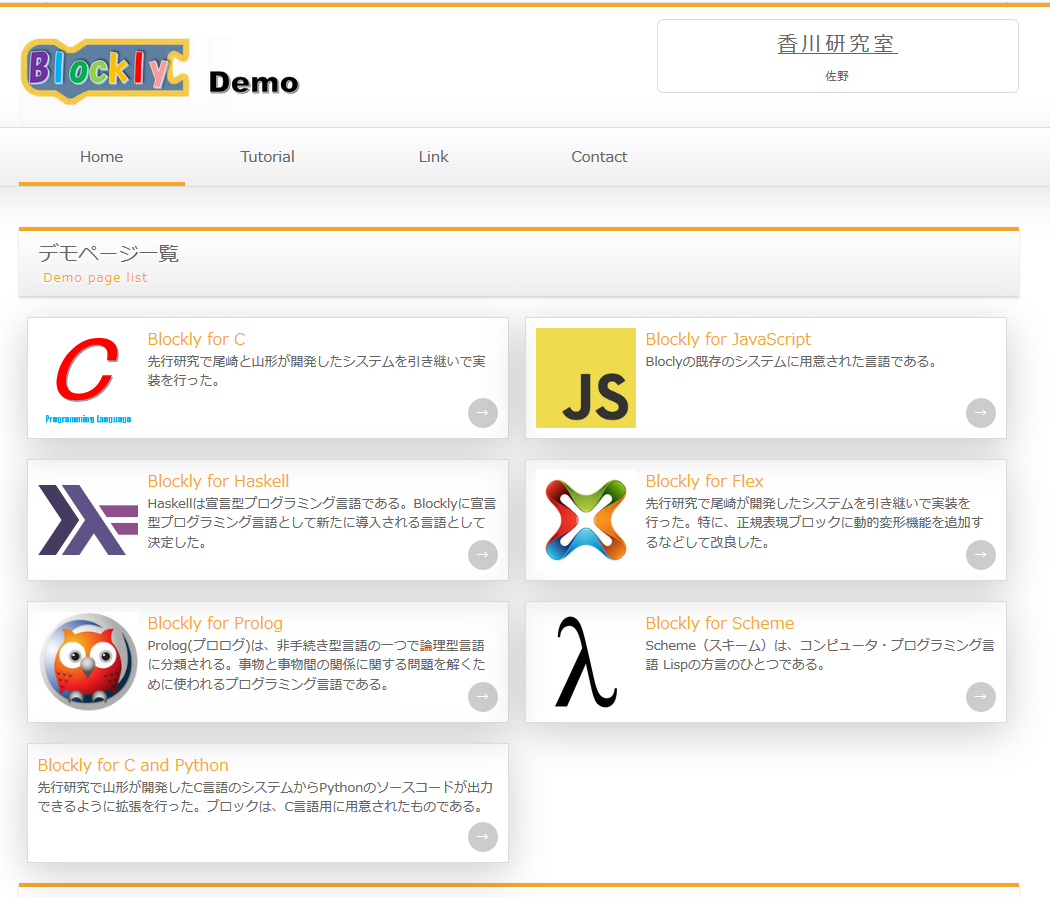
\includegraphics[scale=0.5]{img/index.PNG}
\caption{索引ページ}%
\label{fig:index}
\end{center}%
\end{figure}% 
   
   \section{ブロックの作成}

ここでは、本システムで新たに実装したブロックと改善したブロックについて分類ごとに分けて説明する。
   

   \subsection{Blockly for Flex}

本小節では、Blockly for Flex で表現できる文法を先に説明し、その後に新たに実装したブロックについて説明する。

\begin{itemize}

\item Blockly で表現できる正規表現の範囲

- 文字列そのものを表す。以下の記述例は、abc+という4文字を表している。

\shadowbox{
\begin{minipage}[t]{3cm}
\begin{verbatim}
”abc+”
\end{verbatim}
\end{minipage}
}

- 特殊文字を文字そのものにする。以下の記述例は、* という特殊文字を文字化してる。

\shadowbox{
\begin{minipage}[t]{3cm}
\begin{verbatim}
\*
\end{verbatim}
\end{minipage}
}

- 文字の集合を表現する。以下の表記が記述例である。aまたはbまたはcの1文字を表している。

\shadowbox{
\begin{minipage}[t]{3cm}
\begin{verbatim}
[abc]
\end{verbatim}
\end{minipage}
}

- 文字集合の範囲を指定する。以下の記述例は、0から9までの1文字を表している。

\shadowbox{
\begin{minipage}[t]{3cm}
\begin{verbatim}
[0-9]
\end{verbatim}
\end{minipage}
}

- 補集合を指定する。以下の記述例は、数字位階の1文字を表している。

\shadowbox{
\begin{minipage}[t]{3cm}
\begin{verbatim}
[^0-9]
\end{verbatim}
\end{minipage}
}

- 改行を除く任意の文字を表現する。以下の表記が記述例である。

\shadowbox{
\begin{minipage}[t]{3cm}
\begin{verbatim}
.
\end{verbatim}
\end{minipage}
}

- 二者択一を表現する。以下の記述例は、aまたはbの1文字を表している。

\shadowbox{
\begin{minipage}[t]{3cm}
\begin{verbatim}
a|b
\end{verbatim}
\end{minipage}
}

- 選択の任意を表現する。以下の記述例は、abまたはaを表している。

\shadowbox{
\begin{minipage}[t]{3cm}
\begin{verbatim}
ab?
\end{verbatim}
\end{minipage}
}

- 0個以上の繰り返しを表現する。以下の記述例は、aの0個以上の繰り返しを表している。

\shadowbox{
\begin{minipage}[t]{3cm}
\begin{verbatim}
a*
\end{verbatim}
\end{minipage}
}

- 1個以上の繰り返しを表現する。以下の記述例は、aの1個以上の繰り返しを表している。

\shadowbox{
\begin{minipage}[t]{3cm}
\begin{verbatim}
a+
\end{verbatim}
\end{minipage}
}

\item 正規表現のブロック群

Blockly for Flex では、先行研究で尾崎が実装したブロックを参考にしながら正規表現のブロックを一新した。ブロックの表現は、実際のFlexの文法の記述形式としている。これでユーザは、構文エラーに悩まされることなくプログラミングを行うことができる。以下の図\ref{fig:flex_RE_blocks}に、正規表現のブロック群を示す。

\begin{figure}[h]
\begin{center}
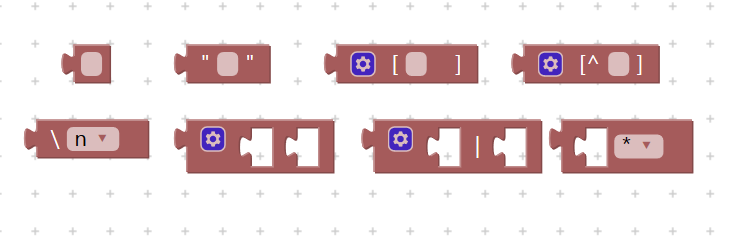
\includegraphics[scale=0.8]{img/flex_RE_blocks.PNG}
\caption{正規表現ブロック群}%
\label{fig:flex_RE_blocks}
\end{center}%
\end{figure}% 

\item 文字クラスブロック

文字クラスブロックには、新たな動的変形機能が実装されており、flexシステムの正規表現ブロックカテゴリで用意されている。以下の図\ref{fig:character_class_block}に、文字クラスブロックの動的変形機能を示す。

正規表現初心者は、「[」と「]」の間に正規表現を書き込もうとするのはよくある間違いである。実際には、「\textasciicircum」や「-」、「\textbackslash 」、「]」以外の文字は「[」と「]」の間に特別な意味を持たないため、「(」、「)」などの正規表現の特殊文字でさえも「)」、「\textbar」および「*」は文字自体として扱われる。この間違いを避けるために、文字クラス用に提案されたブロックでは、内部で他の正規表現を許可せずに、動的変形ダイアログで3種類のサブブロックを提供している。範囲ブロックをサブブロックとして接続すると、2つの入力フォームが表示され、親ブロックに文字範囲を入力できる。単一文字のサブブロックを追加する場合、親ブロックに任意の単一文字を入力できる。特殊文字サブブロックの場合、5つの特殊文字から選択できるドロップダウンメニューが表示される。

\begin{figure}[h]
\begin{center}
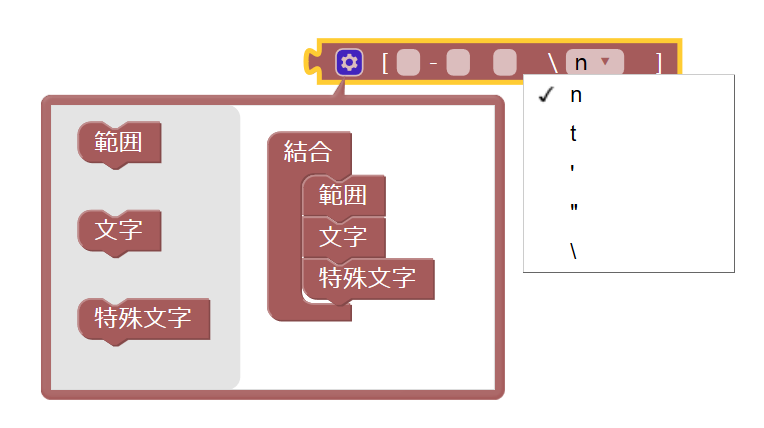
\includegraphics[scale=0.8]{img/character_class_block.png}
\caption{文字クラスブロック}%
\label{fig:character_class_block}
\end{center}%
\end{figure}% 

\item 正規表現連結ブロック

FlexのBlocklyブロックのもう1つの問題は、バイナリ演算子に2値ブロックのみを使用すると、ブロックが深く入れ子になりすぎて表示に収まらないことである。 Flexでは、連結(単純に並置される)と代替(「\textbar」演算子で表される)が正規表現で非常に頻繁に使用されるため、この問題は深刻である。これを解決するために、\ref{fig:flex_connection_block}の連結ブロックでは、値入力の数をMutatorダイアログで増やして、複数連結または複数代替正規表現を表すことができる。繰り返しブロックでは、プルダウンメニューで繰り返しの意味を示す演算子「+」、「*」、「?」から演算子を選択できる。提案されたブロックは、実際のFlexキーワードと演算子記号を使用する。これにより、ユーザーは構文エラーに煩わされることなくプログラミングできる。

\begin{figure}[h]
\begin{center}
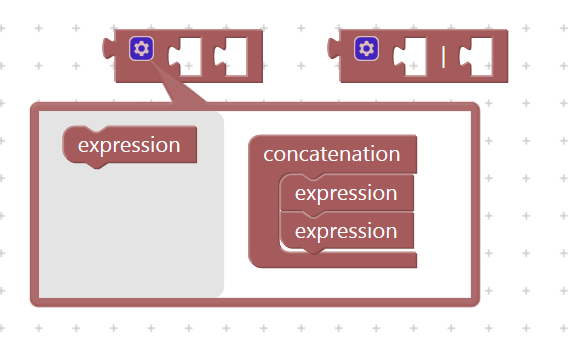
\includegraphics[scale=0.8]{img/flex_connection_block.png}
\caption{正規表現連結ブロック}%
\label{fig:flex_connection_block}
\end{center}%
\end{figure}% 

\end{itemize} 

   \subsection{Blockly for Haskell}

本小節では、Blockly for Haskell で表現できる文法をソースコードを例に説明し、その後に新たに実装したブロックと改善したブロックについて説明する。Haskellでは、関数におけるパターンマッチングによる場合分けで処理を定義することができ、引数がリストの場合にも対応した。また、内包表記を扱ったリストもブロックで表現可能である。

\begin{itemize}

\item リスト内包表記のソースコード例

Haskellは純粋に関数型プログラミング言語であり、手続き型言語とはかなり異なる構文を持っている。リスト内包表記のソースコード例を以下に示す。

\begin{lstlisting}[basicstyle=\ttfamily\footnotesize]
foo n = [(x、y)| x <-[0..n]
                 , y <-[x..n]
                 , mod(x + y)2 == 1]
\end{lstlisting}

ここで、x \verb|<|-[0..n]などの形式はジェネレーターである。これは、変数xがリスト[0..n]の要素の1つにバインドされていることを意味する。mod(x + y)2 == 1などのブール式は、ガードと呼ばれる。変数間で保持される条件を表す。したがって、式foo 3はリスト[(0,1),(0,3),(1,2),(2,3)]に評価される。

\item リスト内包表記ブロック

2つの図共に左図が、リスト内包表記ブロックに何も接続していない初期状態で、右図がさきほどのHaskellのソースコード例をリスト内包表記ブロックを使って接続した例である。以下の図\ref{fig:inner_table_old}に内包表記ブロックの改善前の状態、図\ref{fig:inner_table_new}に内包表記ブロックの改善後の状態をを示す。

Blockly for Haskell のリスト内包表記カテゴリーで内包表記ブロックを改善して実装した。リスト内包表記のソースコードは、リストの中に1つの式と複数の限定式で記述される。

改善前は、内包表記と書かれた右上のソケットに式を挿入式し、限定式と書かれた箇所の右に複数の限定式を表すブロックを挿入する仕様となっている。しかし、限定式の挿入部分に式ブロックを挿入することができないので黒ブロックで用意して接続部を調整している。この黒ブロックは、XML形式に変換する際に不具合が起こる原因となる。

改善後は、「内包表記 限定式」という表記をなくしてシンプルにした。そして、接続部の調整するブロックを垂直接続から内部接続に変更できるブロックを用意し、XML形式に変換する際に起こる不具合を修正した。

\shadowbox{
\begin{minipage}[t]{6cm}
\begin{verbatim}
[ 式 | 限定式, ... , 限定式 ]
\end{verbatim}
\end{minipage}
}

\begin{figure}[h]
\begin{center}
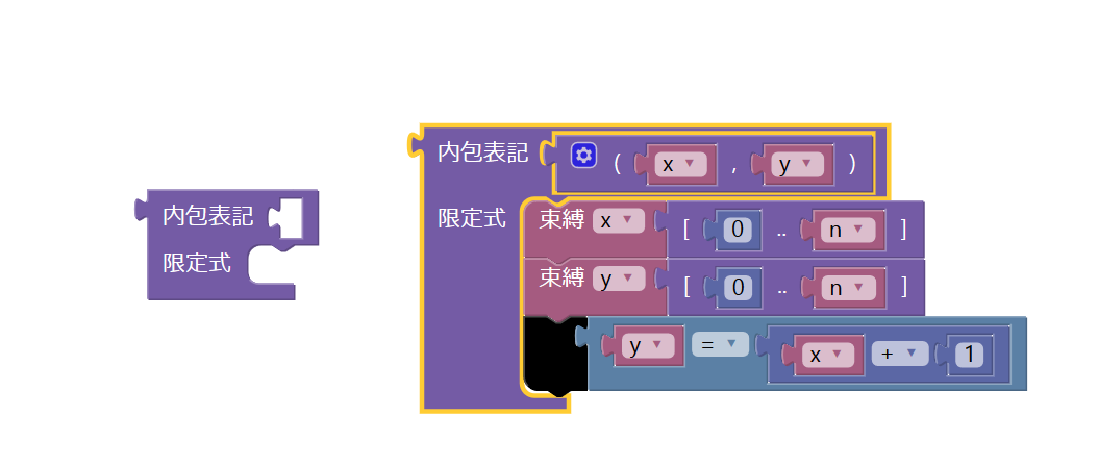
\includegraphics[scale=0.5]{img/inner_table.eps}
\caption{リスト内包表記ブロックの改善前}%
\label{fig:inner_table_old}
\end{center}%
\end{figure}% 

\begin{figure}[h]
\begin{center}
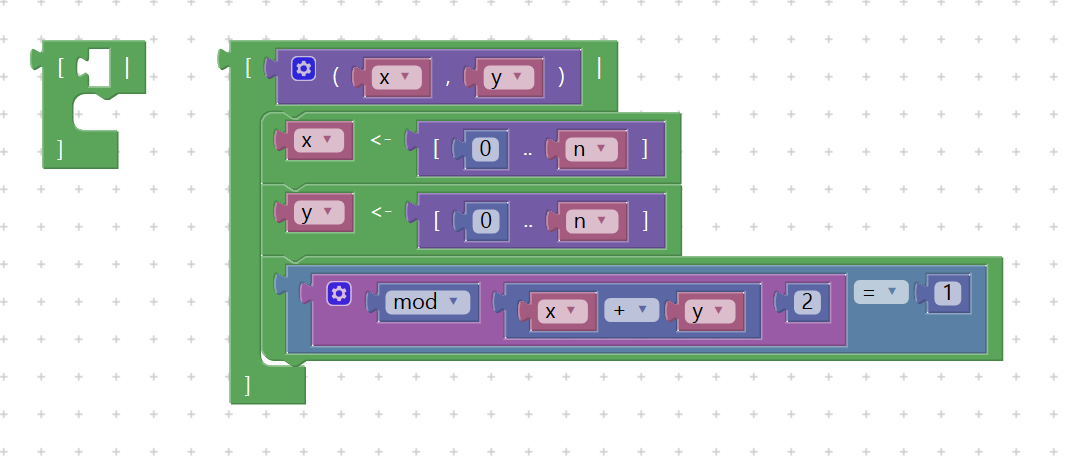
\includegraphics[scale=0.5]{img/inner_table.PNG}
\caption{リスト内包表記ブロックの改善後}%
\label{fig:inner_table_new}
\end{center}%
\end{figure}% 

\item 関数定義ブロック

Blockly for Haskell で関数定義ブロックを改善して実装した。以下の図\ref{fig:haskell_function1}に、関数定義ブロックの改善前の状態を示し、図\ref{fig:haskell_function_new}に、関数定義ブロックの改善後の状態を示す。関数定義ブロックでは、Mutator機能で関数の仮引数を自由に設定することができ、Mutatorダイアログのなかの引数ブロックを結合コンテナブロックに組み立てることで仮引数を調整できる。しかし、改善前の状態では、「式 ===\textgreater」の右の接続部に式を表すブロックを接続し、その下に引数を表すブロックを挿入する仕様だったが、改善後では「=」の左部分のソケットに引数ブロックを「=」右部分に式ブロックを挿入できるように改善した。

\begin{figure}[h]
\begin{center}
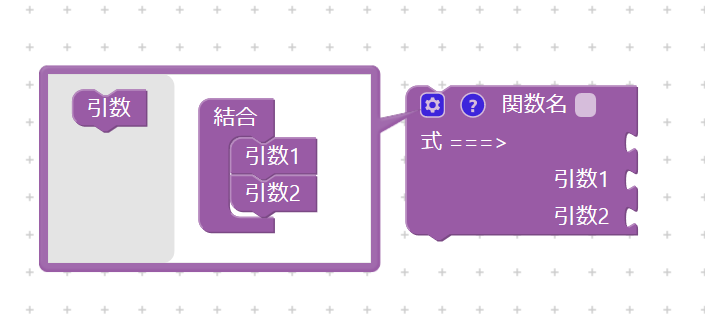
\includegraphics[scale=0.5]{img/haskell_function_old.PNG}
\caption{改善前の関数定義ブロック}%
\label{fig:haskell_function1}
\end{center}%
\end{figure}% 

\begin{figure}[h]
\begin{center}
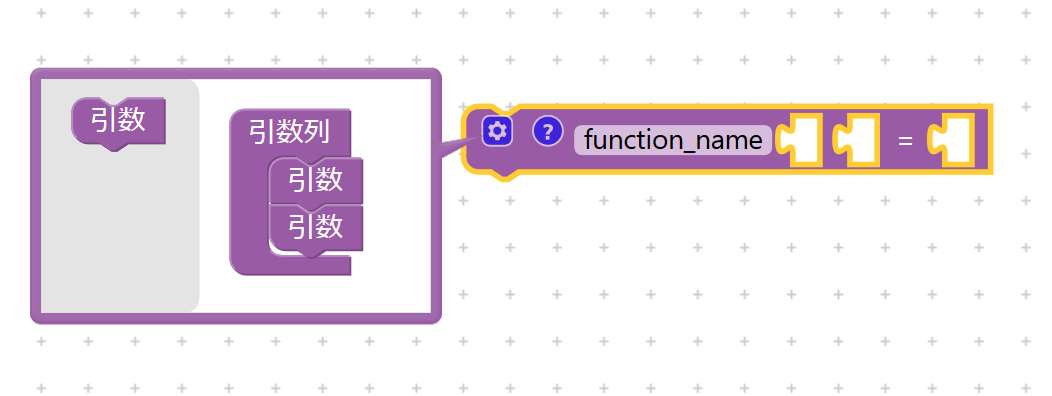
\includegraphics[scale=0.5]{img/haskell_function.PNG}
\caption{改善後の関数定義ブロック}%
\label{fig:haskell_function_new}
\end{center}%
\end{figure}% 

\item 関数呼び出しブロック

Blockly for Haskell で関数呼び出しブロックを改善して実装した。関数呼び出しブロック自身でもMutator機能で引数を調整できるように改善した。以下の図\ref{fig:haskell_function_call_old}に改善前の関数呼び出しブロックを示し、図\ref{fig:haskell_function_call_new}に改善後の関数呼び出しブロックを示す。

\begin{figure}[h]
\begin{center}

\includegraphics[scale=0.5]{img/haskell_function_call.eps}
\caption{改善前の関数呼び出しブロック}%
\label{fig:haskell_function_call_old}
\end{center}%
\end{figure}% 

\begin{figure}[h]
\begin{center}
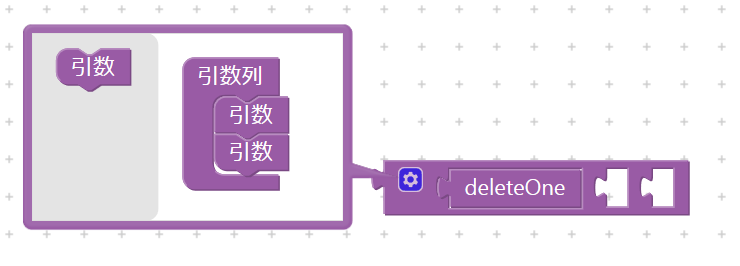
\includegraphics[scale=0.5]{img/haskell_function_call_new.PNG}
\caption{改善後の関数呼び出しブロック}%
\label{fig:haskell_function_call_new}
\end{center}%
\end{figure}% 

\item 関数定義ブロックと関数呼び出しブロックの接続例

以下のソースコードを関数定義ブロックと関数呼び出しブロックを使って接続する。deleteOne関数は、指定された要素(第1引数)をリスト(第2引数)の要素から見つけ出し消去する関数である。
\begin{lstlisting}[basicstyle=\ttfamily\footnotesize]
deleteOne _ [] = []
deleteOne n (x:xs) = if n == x then xs else x:deleteOne n xs
\end{lstlisting}

以下の図\ref{fig:haskell_function_example}に、上記のHaskellソースコードを改善した関数定義ブロックと関数呼び出しブロックで接続した例を示す。

今回の例のパターンマッチングでは、第1仮引数は任意の数で、第2仮引数は任意のリストである。その際のリストの先頭要素をx、それ以降のリストをxsを表す。式と書かれた接続部では、もしも実行ブロックを接続し、もしも任意の数nとリストの先頭要素xが等しければリストxsを返し、それ以外なら先頭要素がxでそれ以降の要素は関数deleteOneを呼び出したリストを返す。リストの中で呼び出した関数deleteOneの第1実引数はn、第2実引数はxsである。

\begin{figure}[h]
\begin{center}
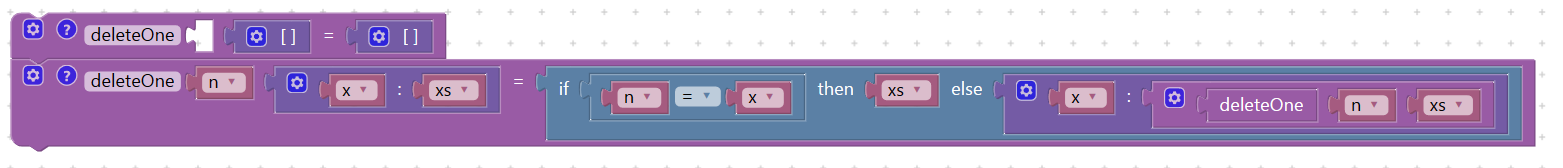
\includegraphics[scale=0.5]{img/haskell_function_example.PNG}
\caption{改善後の関数ブロックと関数呼び出しブロックの接続例}%
\label{fig:haskell_function_example}
\end{center}%
\end{figure}% 

\item 標準関数ブロック

システム利用者から、「標準関数を扱えるブロックが欲しい」といった要望が複数寄せられたので、Blockly for Haskell で、標準関数ブロックを実装した。以下の図\ref{fig:haskell_standard_functions}に、標準関数ブロックのイメージを示す。標準関数ブロックは、標準関数カテゴリーで6種類用意されているのが、標準関数ブロックの選択フォームではそれ以上の種類の標準関数を選択することができる。そして、Mutator機能で標準関数にあった引数の数を調整することができる。

\begin{figure}[h]
\begin{center}
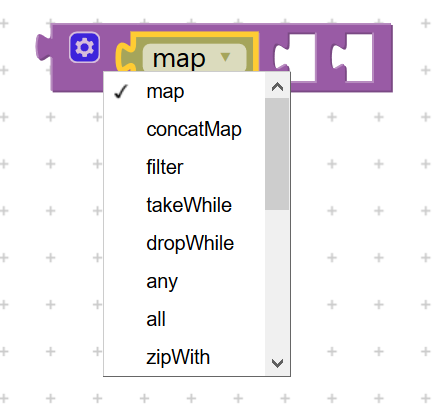
\includegraphics[scale=0.5]{img/haskell_standard_functions.PNG}
\caption{Haskell の標準関数ブロック}%
\label{fig:haskell_standard_functions}
\end{center}%
\end{figure}% 

\end{itemize} 

   \subsection{Blockly for Prolog}
   
\begin{itemize}   

\item Prolog コードの説明

Prologのプログラムは次の3つの要素から成る。

事実: 事物とその関係についていくつかの事実を宣言すること。

規則: 事物とその関係についての規則を定義すること。

質問: 事物とその関係について質問すること。

以下は、徳川家の家系図をPrologのソースコードを示している。1行目から10行目は事実で、12行目から14行目は規則で、16行目は質問にあたる。事実と規則は、それぞれで書き方が違うため、既存にある関数ブロックに切り替え機能を付けて動的変形できるように実装する必要がある。
また、規則の部分の「X」、「Y」、「Z」にあたるものは既存の変数ブロックで扱えるが、事実の部分の「hideyasu」、「ieyasu」、「yorifusa」にあたるものは新たにブロックを定義する必要がある。
\begin{lstlisting}[basicstyle=\ttfamily\footnotesize]
child(hideyasu,ieyasu).
child(hidetada,ieyasu).
child(yoshinao,ieyasu).
child(yoshinobu,ieyasu).
child(yorifusa,ieyasu).
child(iemitsu,hidetada).
child(tadanaga,hidetada).
child(masayuki,hidetada).
child(ietsuna,iemitsu).
child(tsunayoshi,iemitsu).

grand_child(X,Z) :-
    child(X,Y),
    child(Y,Z).

?- grand_child(X,ieyasu).
\end{lstlisting}

以下の図\ref{fig:prolog_blocks_example}に、上記のPrologソースコードを新しく実装したブロックで接続した例を示す。

\begin{figure}[h]
\begin{center}
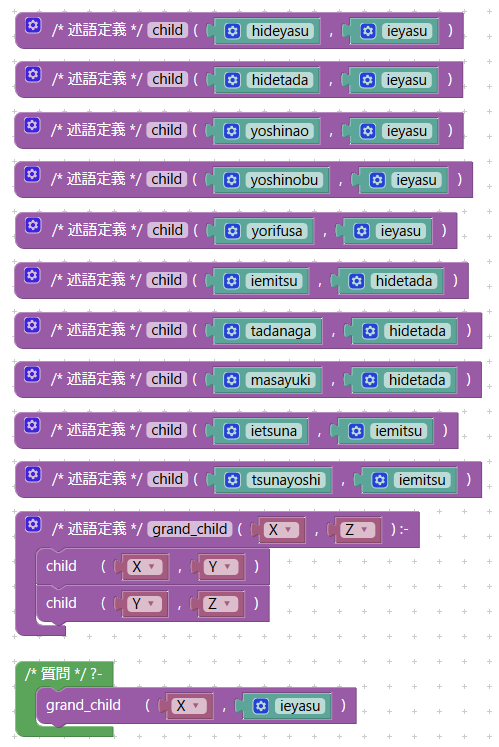
\includegraphics[scale=0.5]{img/prolog_blocks_example.PNG}
\caption{Prologソースコードを新しく実装したブロックで接続した例}%
\label{fig:prolog_blocks_example}
\end{center}%
\end{figure}% 

\item 述語定義ブロック

Blockly for Prolog の述語カテゴリーに述語定義ブロックを実装した。述語定義ブロックでは、事物とその関係についての事実を宣言したり、事物とその関係についての規則を定義することができる。入力フォームで事実名または規則名を入力し、Mutator機能で引数ブロックを調整することで事物の数を設定し、「ゴールを許す」のチェックの有無でそのブロックが事実を表すのか規則を表すのかを切り替えする。事実は必ずしも関係だけを表すものではなく、事物の性質を表す場合もある。規則を表す場合は、「ゴールを許す」にチェックをつけ述語定義ブロックの内側に事物の関係を表すブロックを接続する。以下の図\ref{fig:prolog_predicate_definition}の左側のブロックは規則を表す場合の述語定義ブロックで、右側のブロックは事実を表す場合の述語定義ブロックである。

\begin{figure}[h]
\begin{center}
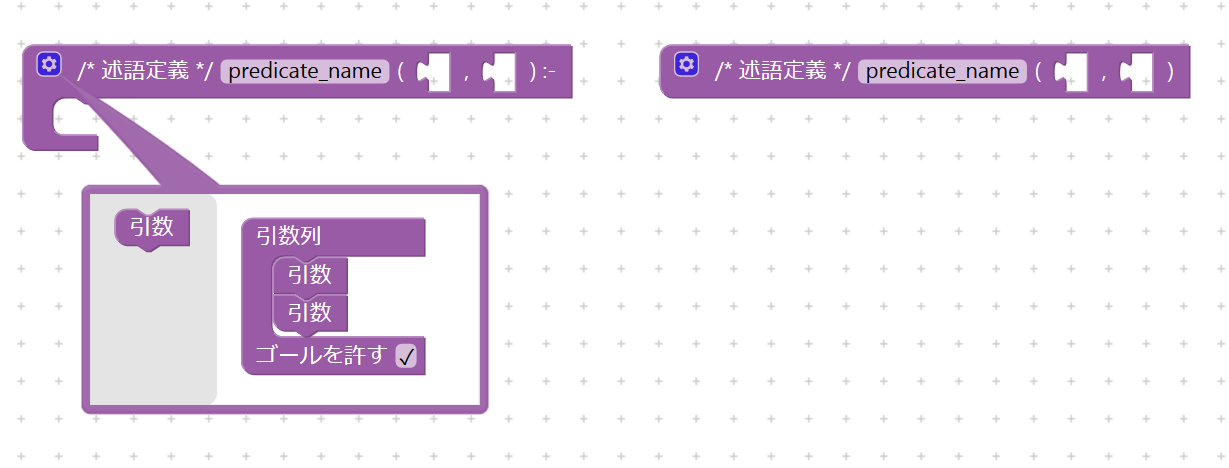
\includegraphics[scale=0.5]{img/prolog_predicate_definition.PNG}
\caption{述語定義ブロック}%
\label{fig:prolog_predicate_definition}
\end{center}%
\end{figure}%

\item 述語ブロック

Blockly for Prolog の述語カテゴリーに述語ブロックを実装した。述語ブロックでは、述語定義ブロックで定義された事実や規則を継承したい場合に使用する。述語定義ブロックをワークスペース部に設置したときに述語カテゴリーで選択できるようになり、ワークスペース部に同一の名称の述語定義ブロックが削除されると同時に述語ブロックも削除される。以下の図\ref{fig:prolog_predicate}に述語ブロックのイメージを示す。

\begin{figure}[h]
\begin{center}
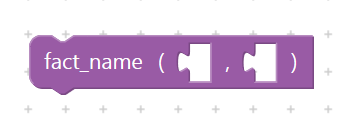
\includegraphics[scale=0.8]{img/prolog_predicate.PNG}
\caption{述語ブロック}%
\label{fig:prolog_predicate}
\end{center}%
\end{figure}% 

\item ファンクター定義ブロック

Blockly for Prolog のファンクターカテゴリーにファンクター定義ブロックを実装した。以下の図\ref{fig:prolog_functor}に、新たに実装したファンクター定義ブロックのイメージを示す。ファンクター定義ブロックでは、ある事物を定義することができる。入力フォームで事物の名称を入力し、述語定義ブロックのソケットに接続することで事物の関係や性質を表す。

\begin{figure}[h]
\begin{center}
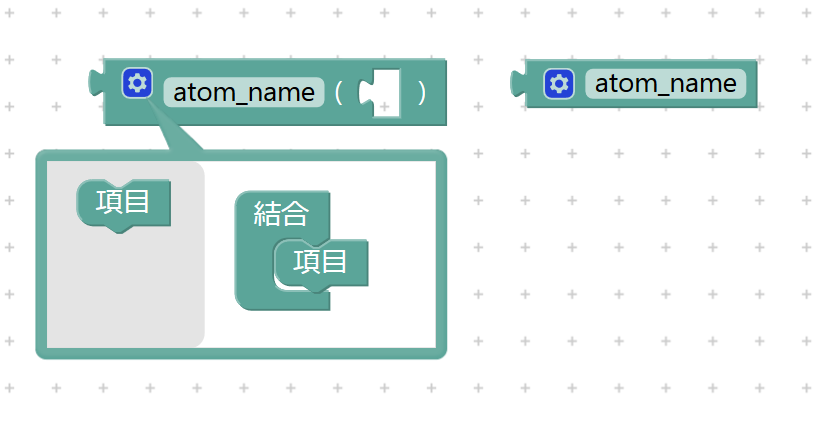
\includegraphics[scale=0.5]{img/prolog_functor.PNG}
\caption{ファンクター定義ブロック}%
\label{fig:prolog_functor}
\end{center}%
\end{figure}% 

\item 質問ブロック

Blockly for Prolog の質問カテゴリーに質問ブロックを実装した。Prologでは、いくつかの事実があるとき質問することができる。質問ブロックの内側には、事物の関係を表す述語ブロックを接続する。以下の図\ref{fig:prolog_question}の左側は質問ブロックに何も接続されていない状態で、右側は質問ブロックの接続例である。

\begin{figure}[h]
\begin{center}
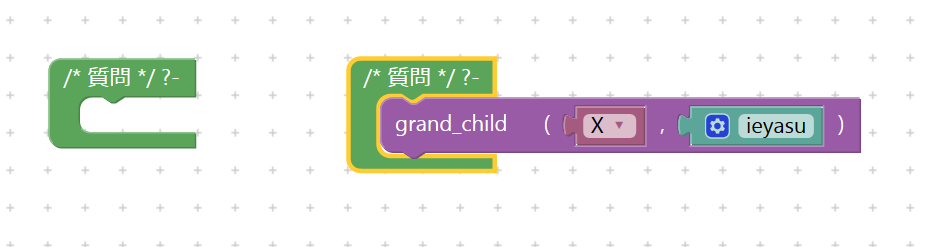
\includegraphics[scale=0.5]{img/prolog_question.PNG}
\caption{質問ブロック}%
\label{fig:prolog_question}
\end{center}%
\end{figure}% 

\end{itemize} 

   \subsection{Blockly for Scheme}
   
\begin{itemize}   

\item Scheme コードの説明

Scheme は、繰り返しやループ構造をすべて再帰呼び出しによって実現できる。ほとんどのプログラミング言語でサポートされている while や for といった制御構造がない。よって、Scheme ではこれらと同じ機能をすべて再帰呼び出しによって実現することができる。

Scheme では関数もひとつのオブジェクトなので、関数を定義するときも変数の定義と同じ define を使う。ただしこの場合は変数に数値型や文字列型オブジェクトを束縛するのではなくて、関数型オブジェクトを束縛します。しかし、関数型オブジェクトはユーザが直接キーボードから入力することはできない。このために Scheme には lambda という特別な構文が用意されている。

以下は、Scheme のソースコードを示している。increase関数は指定された定数(第1引数)から昇順に1ずつ加算していき、decrease関数は指定された定数(第1引数)から1ずつ減算していく。既存の関数ブロックを改善する必要があり、「begin」や「call-with-current-continuation」、「lambda」などの構文は、新たなブロックを定義する必要がある。

\begin{lstlisting}[basicstyle=\ttfamily\footnotesize]
(define (increase n k)
 (if (> n 10) #f (begin (display " i:") (display n) (increase (+ n 1) (call-with-current-continuation k)))))

(define (decrease n k)
 (if (< n 0) #f (begin (display " d:") (display n) (decrease (- n 1) (call-with-current-continuation k)))))

(increase 0 (lambda (k) (decrease 10 k)))
\end{lstlisting}

以下の図\ref{fig:scheme_blocks_example}に、上記のSchemeソースコードを新しく実装したブロックで接続した例を示す。

\begin{figure}[h]
\begin{center}
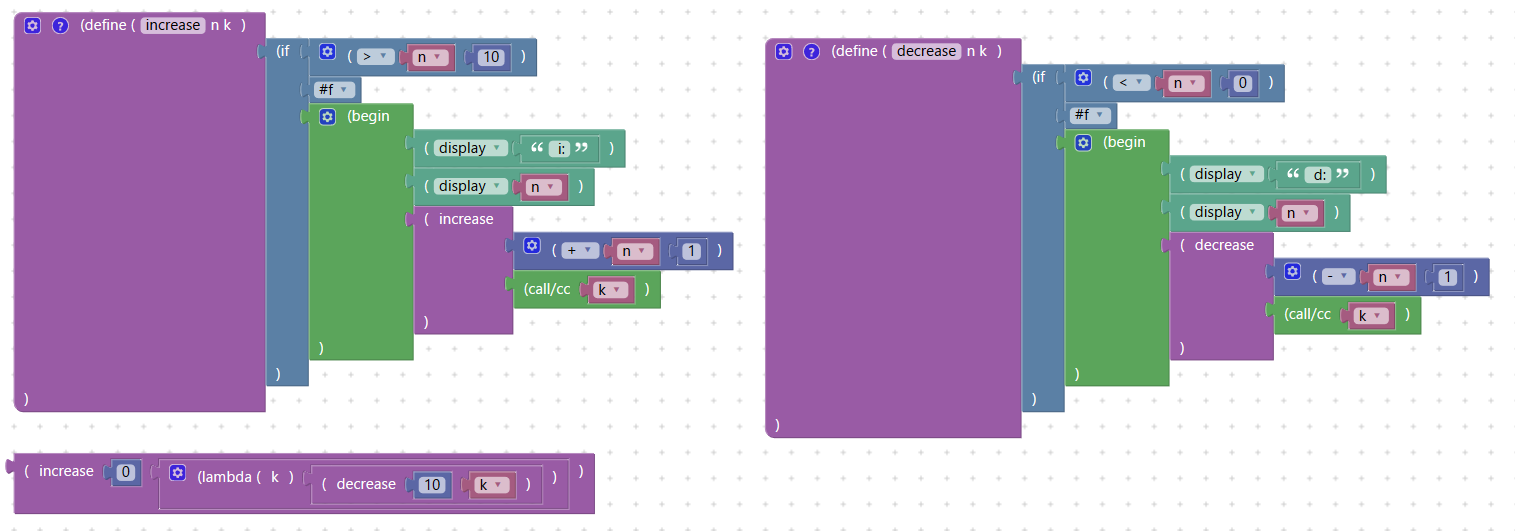
\includegraphics[scale=0.5]{img/scheme_blocks_example.PNG}
\caption{Schemeソースコードを新しく実装したブロックで接続した例}%
\label{fig:scheme_blocks_example}
\end{center}%
\end{figure}% 


\item beginブロック

Blockly for Scheme の制御カテゴリーにbeginブロックを実装した。Mutator機能でvalue inputを調整することで式の数を自由に設定できる。beginブロックは、begin構文を表す。begin構文は、複数の式を1つにまとめることができる。beginは与えられた式を前から順番に評価していき、最後の式の値を返す。以下の図\ref{fig:scheme_begin}にbeginブロックのイメージを示す。

\begin{figure}[h]
\begin{center}
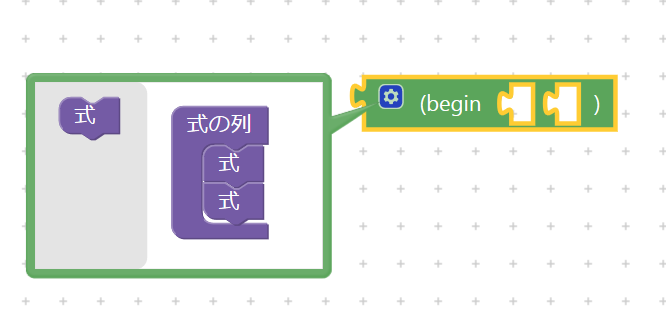
\includegraphics[scale=0.5]{img/scheme_begin.PNG}
\caption{beginブロック}%
\label{fig:scheme_begin}
\end{center}%
\end{figure}% 

\item 変数束縛ブロック

Blockly for Scheme の制御カテゴリーに変数束縛ブロックを実装した。Mutator機能でvalue inputの数を調整することで式の数を自由に設定できる。変数束縛ブロックでは、選択フォームでlet式、let*式、letrec式を選択でき、いずれの構文も値を変数に束縛するために用いられる。以下の図\ref{fig:scheme_binding}の左側は、変数束縛ブロックのイメージで、右側は変数束縛ブロックのMutator機能と選択フォームのイメージである。

\begin{figure}[h]
\begin{center}
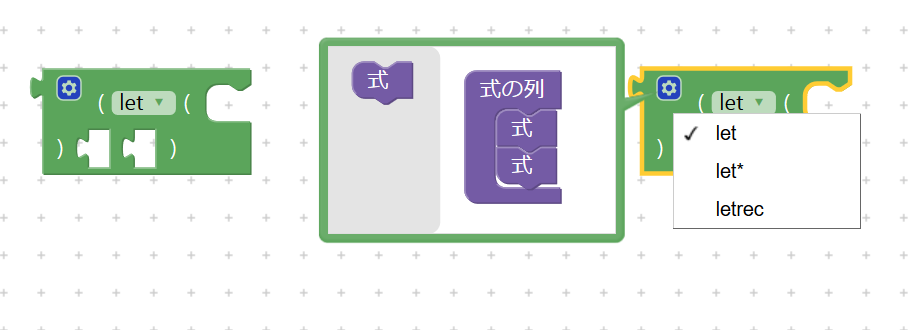
\includegraphics[scale=0.5]{img/scheme_binding.PNG}
\caption{変数束縛ブロック}%
\label{fig:scheme_binding}
\end{center}%
\end{figure}% 

\item call/ccブロック

lockly for Scheme の制御カテゴリーにcall/ccブロックを実装した。call/ccとは、call-with-current-continuation という scheme の手続きで、「現在の継続(current continuation)を生成し、それを関数に渡してその関数を実行する」ものである。以下の図\ref{fig:scheme_callcc}にcall/ccブロックのイメージを示す。

\begin{figure}[h]
\begin{center}
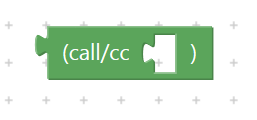
\includegraphics[scale=0.8]{img/scheme_callcc.PNG}
\caption{call/ccブロック}%
\label{fig:scheme_callcc}
\end{center}%
\end{figure}% 

\item lambdaブロック

lockly for Scheme の関数カテゴリーにlambdaブロックを実装した。lambdaは手続きを新たに定義し、その手続きを表す値を返す構文である。Mutator機能により引数と式の数を設定できる。Mutator機能の入力名ブロックの入力フォームで引数の名前を入力し、小窓のワークスペース部の入力の真下に接続して引数を決定する。式の列の真下に式ブロックを接続して式の数を決定する。以下の図\ref{fig:scheme_lambda}にlambdaブロックのイメージを示す。

\begin{figure}[h]
\begin{center}
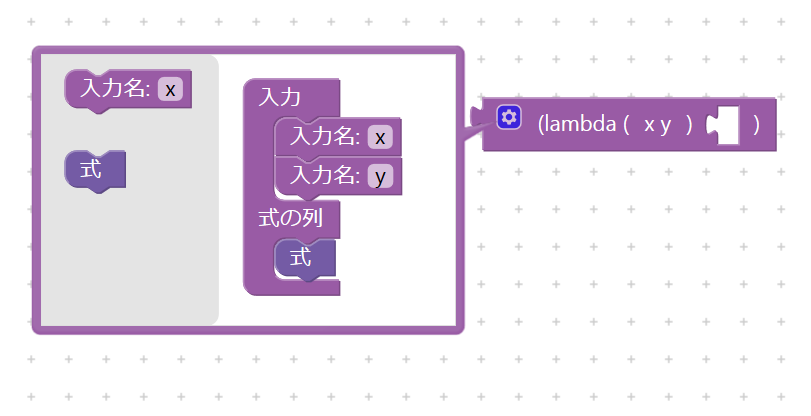
\includegraphics[scale=0.8]{img/scheme_lambda.PNG}
\caption{lambdaブロック}%
\label{fig:scheme_lambda}
\end{center}%
\end{figure}% 

\item 関係定義ブロックと関数ブロック

Blockly for Scheme の関数カテゴリーに関数定義ブロックと関数ブロックを実装した。関数定義ブロックのMutator機能により引数と式の数を設定できる。Mutator機能の仕様は、lambdaブロックと同じである。以下の図\ref{fig:scheme_func}に関数定義ブロックと関数ブロックのイメージを示す。

\begin{figure}[h]
\begin{center}
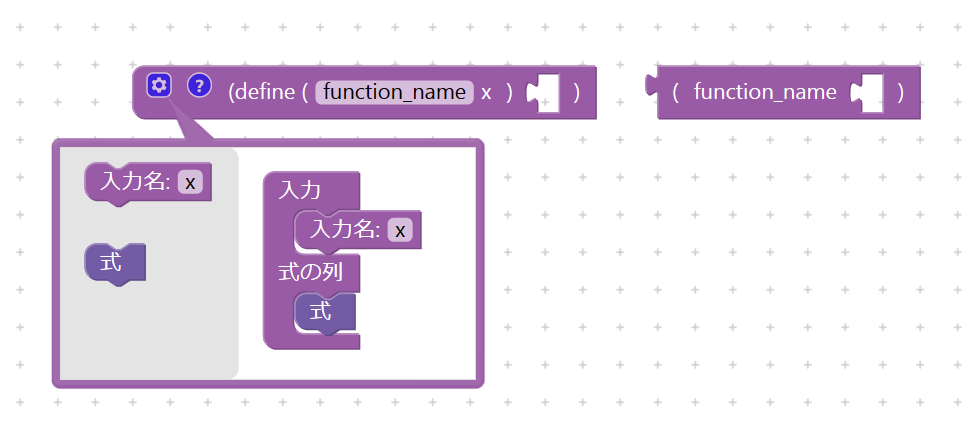
\includegraphics[scale=0.5]{img/scheme_func.PNG}
\caption{関数定義ブロックと関数ブロック}%
\label{fig:scheme_func}
\end{center}%
\end{figure}% 

\end{itemize} 

   \subsection{Haskell と Prolog における関数ブロック}
   
既存のBlocklyに用意されてある関数ブロックは、入力フォームにおいて関数名が別の関数ブロックの関数名と重複する場合は強制的に名称が変更される。しかし、HaskellやPrologの文法は同じ関数を扱う場合があるので、HaskellとProlog言語のシステムで実装した関数ブロックでは、重複した場合でも関数名が変更されない仕様にした。

   \section{Blocky C and Python}
   
本システムを実装する際の当初の目標は、先行研究で山形が開発したC言語のシステムを参考にPythonのコード入力でブロックを生成することであったが、時間の都合上、Pythonのソースコードを出力するまでに至った。ブロックは、C言語用に用意されたものである。コードタブをクリックして、テキストベースでC言語ソースコードを直接入力すれば、そのコードに対応したブロックが生成されるが、Pythonのソースコードを入力してブロックを生成することはできない。システムを使う流れは、「C言語コード入力 → ブロック生成 → Pythonコード確認」である。

C言語のソースコードから組み立てられたブロックのPythonのコードを確認することで、CとPythonの文法を比較しながら理解することができる。
   
   \section{表記切り替え機能}
   
Flexのブロックに表記切り替え機能を実装した。表記には2つのタイプがある。1つは自然言語表記(日本語表記とも呼ばれる)で、もう1つはプログラミング言語の演算子とキーワードを使用する表記(Flex表記)である。切り替えは、HTMLフォームのselect要素によって実行される。日本語表記では、初心者にとっては表現の意味が理解しやすいので、Flex表記に切り替えることができる。これにより、各ブロック部分の概念と、正規表現の構文との対応を理解することができる。図\ref{fig:switching_ja}は日本語表記、図\ref{fig:switching_flex}はFlex表記を表す。

\begin{figure}[h]
\begin{center}
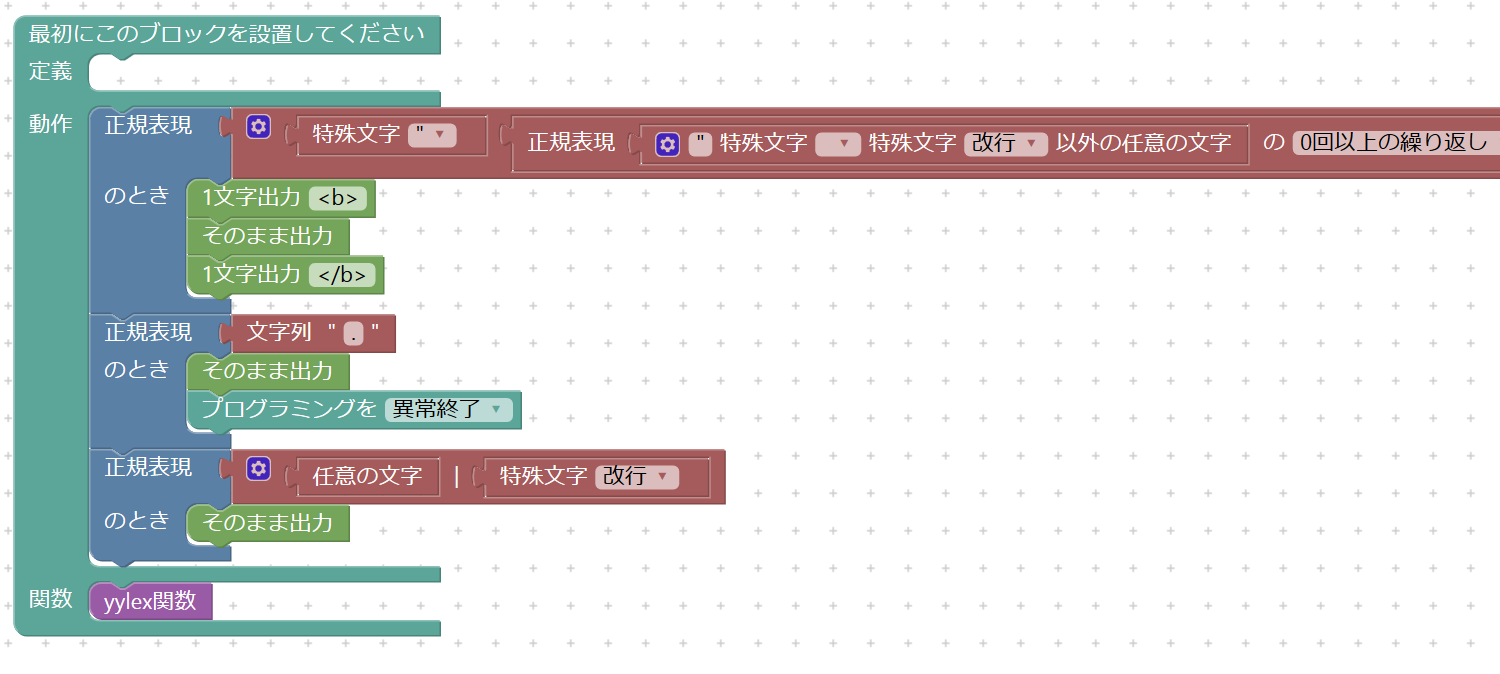
\includegraphics[scale=0.5]{img/switching_ja.PNG}
\caption{日本語表記}%
\label{fig:switching_ja}
\end{center}%
\end{figure}% 

\begin{figure}[h]
\begin{center}
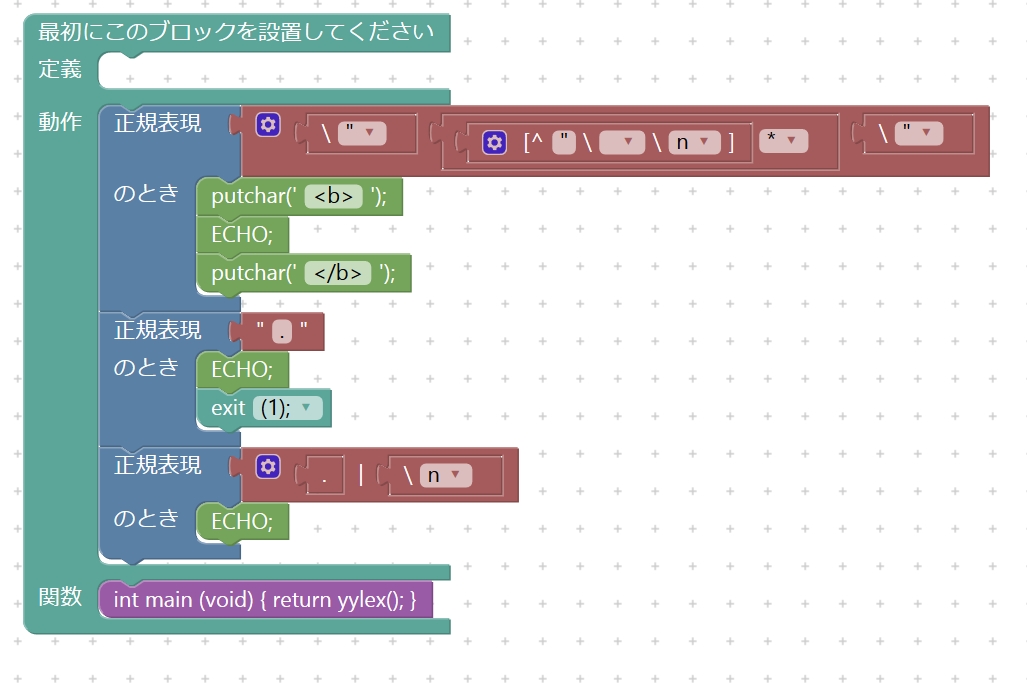
\includegraphics[scale=0.5]{img/switching_flex.PNG}
\caption{Flex表記}%
\label{fig:switching_flex}
\end{center}%
\end{figure}% 

   \section{チュートリアルページ}
   
Blocklyを初めて使う人にスムーズにブロックを組み立ててもらえるように、チュートリアルのWEBページを作成した。システム上部の「システムの使い方について」と書かれたリンク先をクリックすると、チュートリアルのWEBページに移動できるようになってる。図\ref{fig:tutorial}に、チュートリアルのWEBページのイメージを示す。このチュートリアルのページには、以下の機能が詳細に説明されている。

1. システムの概要図と構成

2. ブロックの組み立て方

3. タブの構成

4. サンプルボタン

5. 表記切り替え機能

6. コンテクストメニュー

7. その他のオプション機能

\begin{figure}[h]
\begin{center}
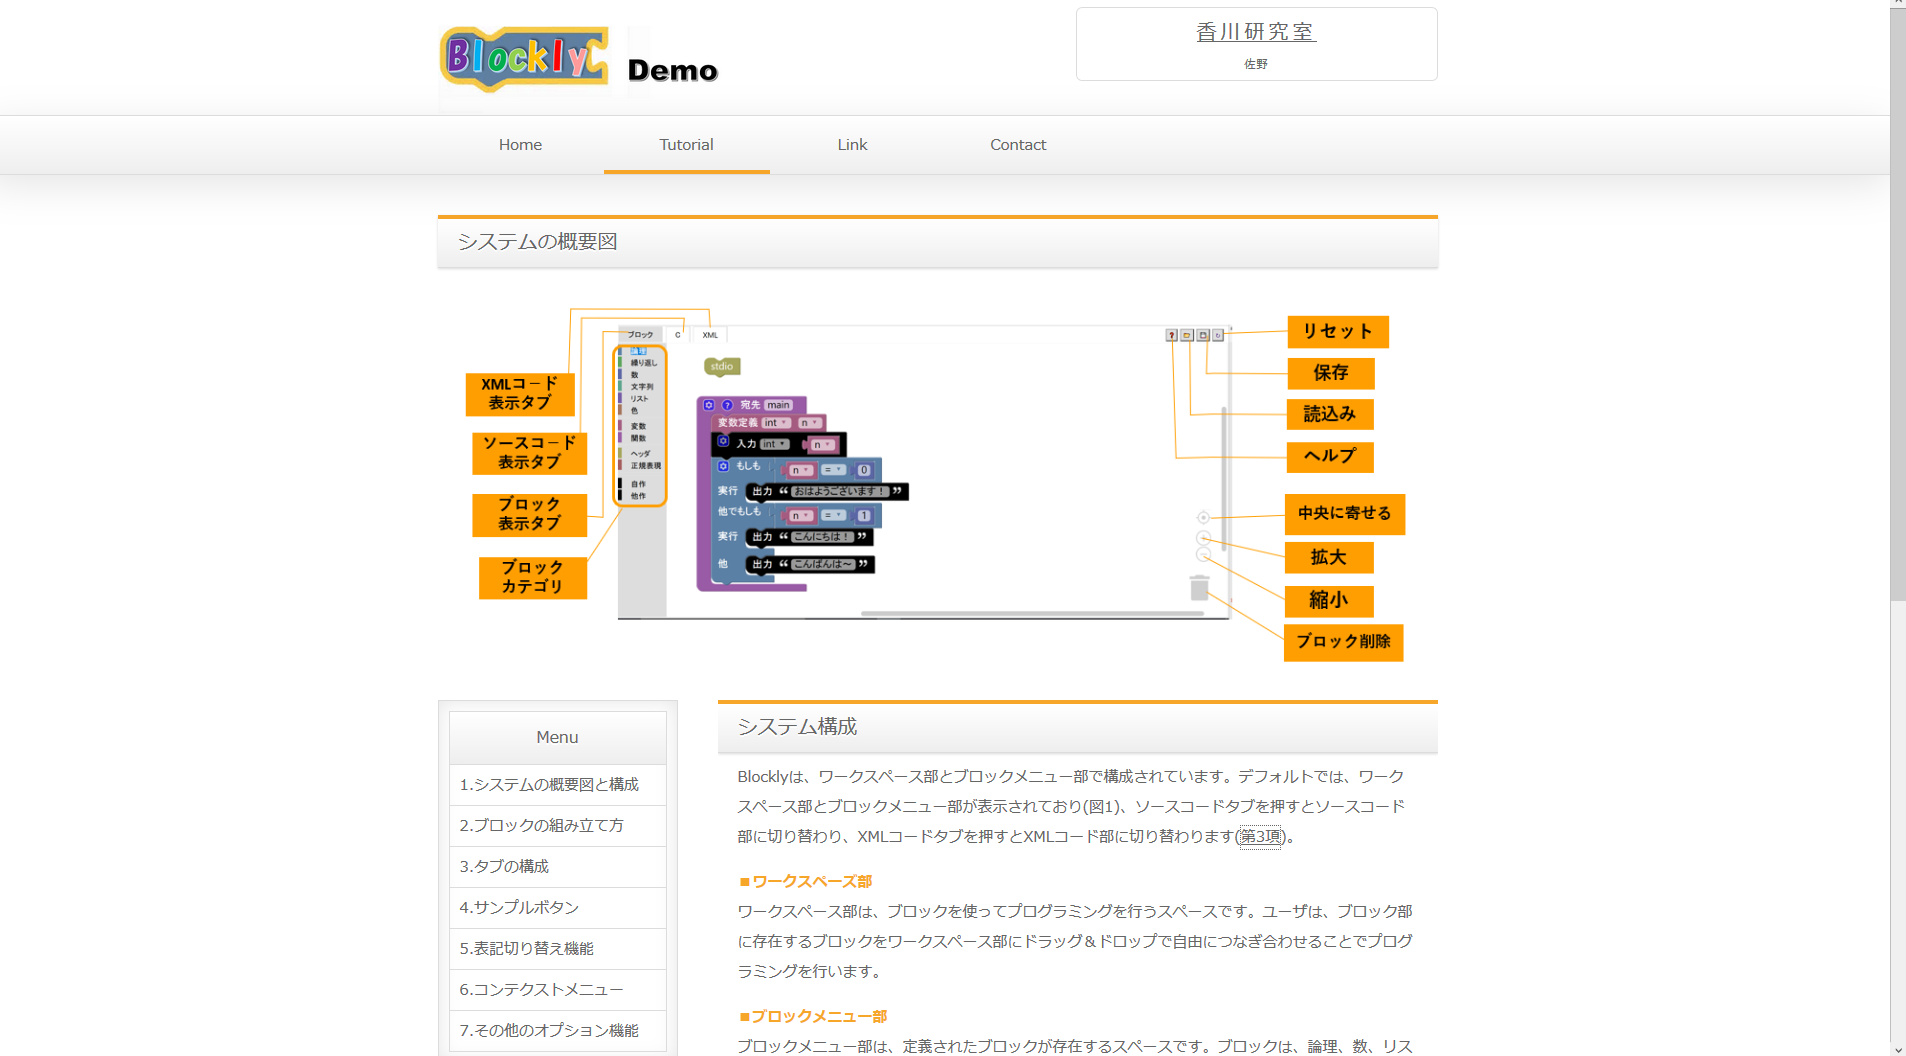
\includegraphics[scale=0.5]{img/tutorial.PNG}
\caption{チュートリアルのWEBページ}%
\label{fig:tutorial}
\end{center}%
\end{figure}% 


   \section{動的変形機能}
   
Mutatorは、Blocklyの既存に用意されている機能だが、本システムではこのMutatoe機能を利用して新たな動的変形機能を実装した。printfブロックに実装されている。そのブロックのイメージは、図\ref{fig:output}である。このブロックは、Blockly for C で用意されている。Mutator機能では、ブロックの左上に歯車マークがあり動的変形機能が実装されていることが分かるが、このブロックは歯車マークがないので、動的変形機能が実装されていることが分からない。しかし、このブロックの入力フォームに図\ref{fig:output2}のような文字列を入力すると、動的変形機能が実装されていることが分かる。これは、入力フォームで"\%"の数を検出して、その数だけvalue inputの数を動的変形機能で増やしている。value inputとは、変数ブロックや数ブロックを挿入できる穴である。検出のタイミングは、入力フォームの中身に変化があるごとに行われる。この機能は、いちいち歯車マークをクリックしてミニワークスペースでブロックを組み立てる必要もないので、動的変形の手間を省きかつ操作もシンプルになっているので、プログラミング学習者の負担を軽減させることができている。

\begin{figure}[h]
\begin{center}

\includegraphics[scale=0.5]{img/output.eps}
\caption{動的変形前のprintfブロック}%
\label{fig:output}
\end{center}%
\end{figure}% 

\begin{figure}[h]
\begin{center}

\includegraphics[scale=0.5]{img/output2.eps}
\caption{動的変形後のprintfブロック}%
\label{fig:output2}
\end{center}%
\end{figure}% 

   \section{サンプル機能}
Blocklyを初めて使う人にとって、ワークスペース部が何も無い状態でブロックを一から組み立てて、実行できるプログラムを完成させることは難しい。そこで、このシステムの初心者が利用しやすくするためにサンプル選択フォームを実装した。図\ref{fig:sample}は、サンプル選択フォームを押したときのワークスペース部のイメージである。WEBページの上部に複数のサンプル用意した。この選択フォームでサンプルを選択することによって、システム開発者側が用意したブロックを一瞬でワークスペース部に表示される。システム初心者は、その完成されたブロックのプログラムをアレンジしながらシステムを理解することができる。

\begin{figure}[h]
\begin{center}
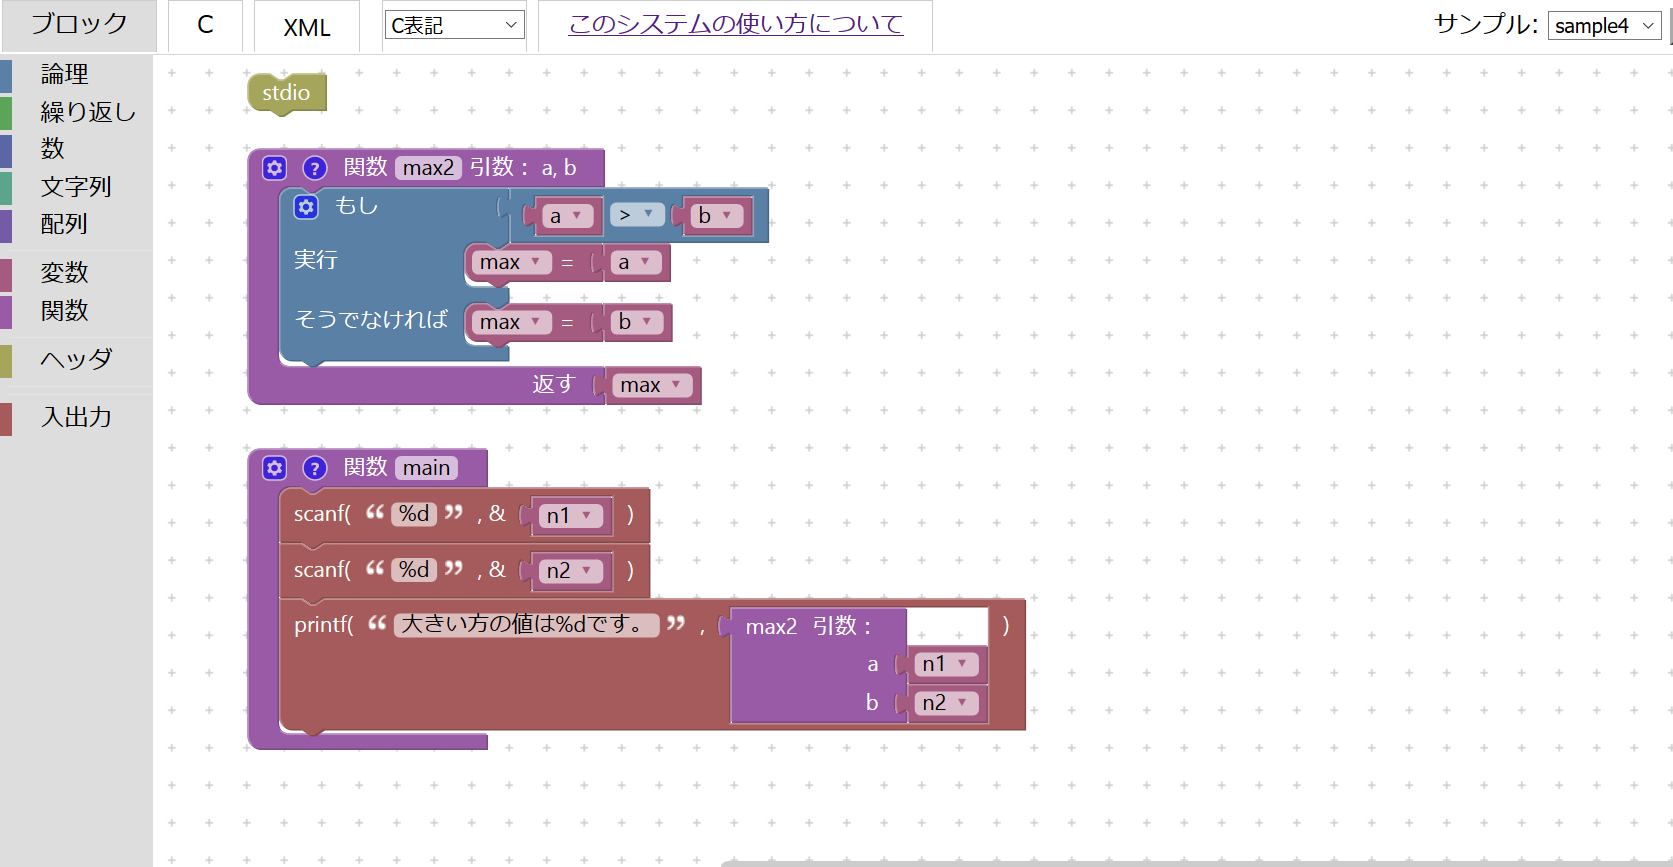
\includegraphics[scale=0.5]{img/sample.PNG}
\caption{サンプルボタンを押したときのワークスペース部}%
\label{fig:sample}
\end{center}%
\end{figure}% 

   \section{実行結果機能}
   
こちらの機能は、Haskell言語のシステム(Blockly for Haskell)とProlog言語のシステム(Blockly for Prolog)、Scheme言語のシステム(Blockly for Scheme)で実装されている。ソースコードタブとXMLコードタブの間に実行結果タブを配置した。ワークスペース部でブロックを組み立てた後、プログラム実行結果タブをクリックすると、図\ref{fig:excution_result}のように組み立てたブロックプログラムからの実行結果が表示される。この実行結果は、過去の結果も表示されるので、それらを消去したい場合は「Clear」ボタンをクリックすると消去される。実行結果は、Haskell の場合は hasteHack.js、Prolog の場合は jsprolog.js、Scheme の場合は biwascheme.js を使って動かしている。

\begin{figure}[h]
\begin{center}
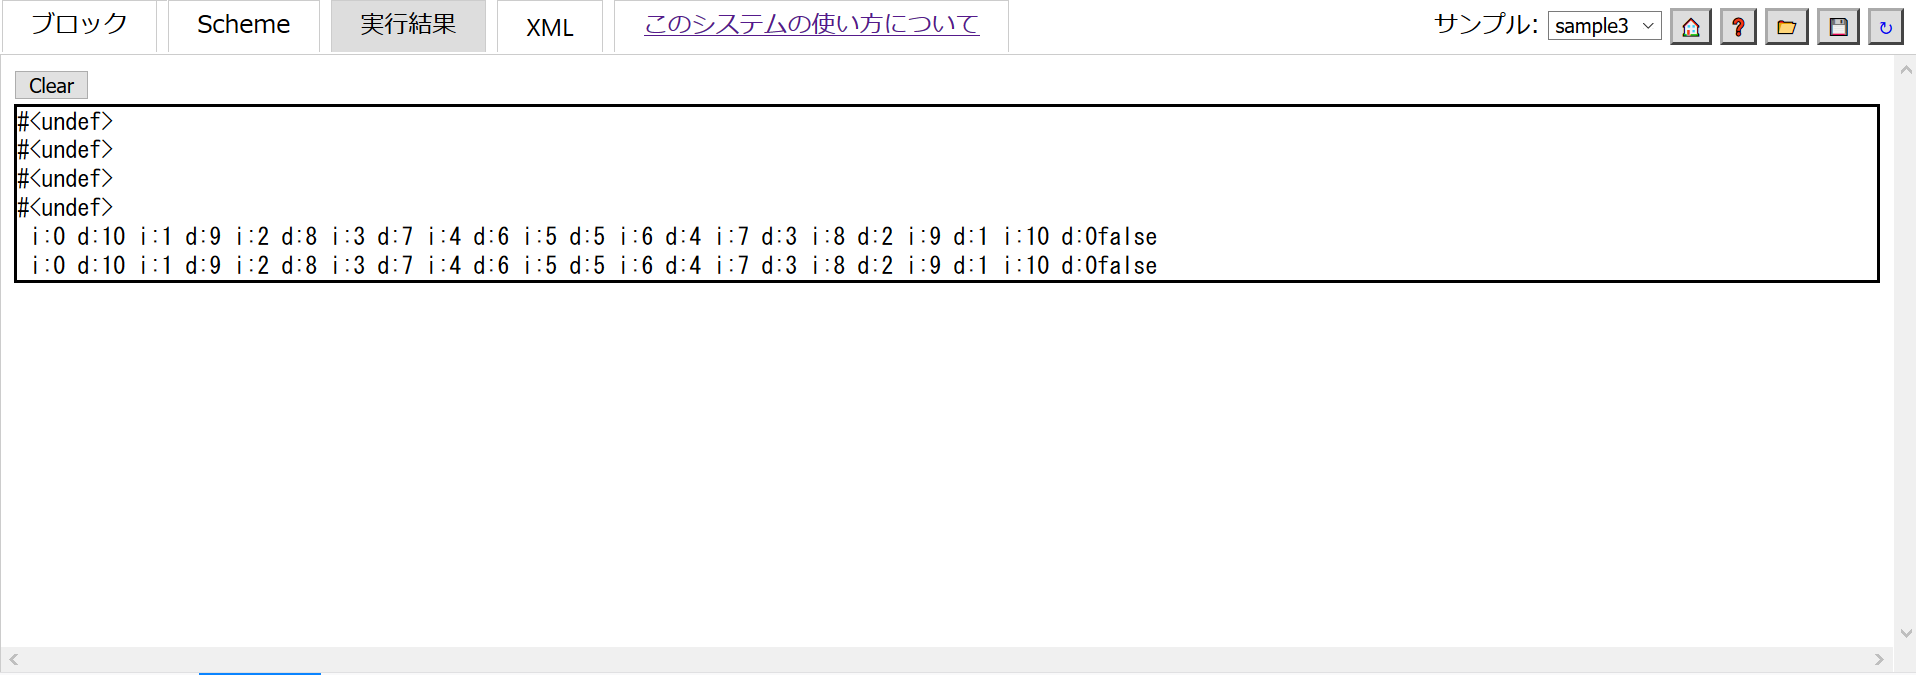
\includegraphics[scale=0.5]{img/execution_result.PNG}
\caption{実行結果のイメージ}%
\label{fig:excution_result}
\end{center}%
\end{figure}% 

   \chapter{評価}
   
   \section{システムの評価概要}
   
本研究では、プログラミング初学者が基礎概念と文法を同時に学習する負担を軽減させるために大学の授業で学ぶプログラミング言語に対応したBlocklyの環境構築を行った。そのため、本研究のBlocklyが初学者にとって有効であるかを調査する必要がある。そこで、各言語のシステムごとに実際に初学者に使用してもらい評価実験を実施した。

   \section{Blockly for Haskell の評価}
   
   		\subsection{評価方法}
Haskell言語システムの評価実験は2回行った。被験者には、実際にHaskellのシステムページにアクセスしてもらい、ほとんど事前説明なしでシステムを利用してもらう。

1回目は、2019年1月に香川研究室の学部生3名を対象に行った。このアンケートを実施した時期は、まだ実行結果機能とチュートリアルのページを実装していない。また、制御カテゴリーとリストカテゴリーにあるブロックは改善前の状態のもので、標準関数カテゴリーのブロックは実装していない状態である。

2回目は、2020年1月に香川研究室の学部生2名を対象に行った。1回目の実験結果から得られたフィードバックをもとに改善されたシステムを利用してもらった。1回目との違いは、チュートリアルのページでブロックの組み立て方を見ることができる点である。

2回の評価実験共に、以下の評価項目に自由に回答する形式で行った。

\begin{itemize}
\item Haskellの学習経験
\item Blockly for Haskell を使用した時間
\item 改善した方がいいと思うところ
\item 意見や感想
\item バグ報告 (非必須)
\item 作成したブロックXMLコード

被験者に組み立てもらったブロックをXMLコードとして全てコピーしてtext形式のアンケートファイルに貼り付けてもらう。XMLコードをもらうことでこちら側で被験者の組み立てたブロックを復元することができる。
\end{itemize} 

		\subsection{1回目の評価結果}

以下は、1回目の評価実験の結果を各評価項目で簡潔にまとめものである。

\begin{itemize}
\item Haskellの学習経験

3人中2人は、Haskellを学習したことのない初学者であり、その他の1人は入門サイトで一通りの構文を学んだ経験があるが、実用的なプログラムは組めない状態である。

\item Blockly for Haskell を使用した時間

15分使用した人から3時間も使用した人まで様々である。

\item 改善した方がいいと思うところ

- 標準ライブラリに定義済みの関数を使えるブロックが欲しい

- 関数の定義が見た目でわかりづらい(特に式===\textgreater)

- Web上で実行結果が表示できるようにしてほしい

- 構文エラーを検出して欲しい

- 関数を呼び出すブロックが右クリックによる派生でないと生成できないのが少々気づきにくい

\item 意見や感想

- 慣れるまでに時間がかかった

- サンプルやチュートリアルを増やしてほしい

-『関数の呼び出し』を行うためのブロックをどうやって生成すればよいのかが分からず、『右クリックを試す』という部分に行く着くまで長い時間を要した

- 何の説明もなしに扱うのは難易度が高いように感じた

\item バグ報告 (非必須)

3点のバグが報告された。これらのバグは現段階では改善されている。バグの詳細な内容については、説明すると長くなるので割愛する。
\item 作成したブロックXMLコード

3人中2人が完成されたHaskellコードのブロックを組み立てることができた。2人の被験者の名称をそれぞれA, Bとする。

Aの完成されたHaskellコードのブロックは図\ref{fig:haskell_experiment_result_a}に、そのHaskellのコードは以下である。myTake関数は、指定された数(第1引数)を配列(第2引数)の先頭要素から取り出して出力する関数である。
\begin{lstlisting}[basicstyle=\ttfamily\footnotesize]
nums = [1..10]

main = do
print nums
print  "の最初の3つは"
print (myTake 3 nums)

myTake 0 _ = []
myTake _ [] = []
myTake n (x:xs) = (x:myTake (n - 1) xs)
\end{lstlisting}

\begin{figure}[h]
\begin{center}
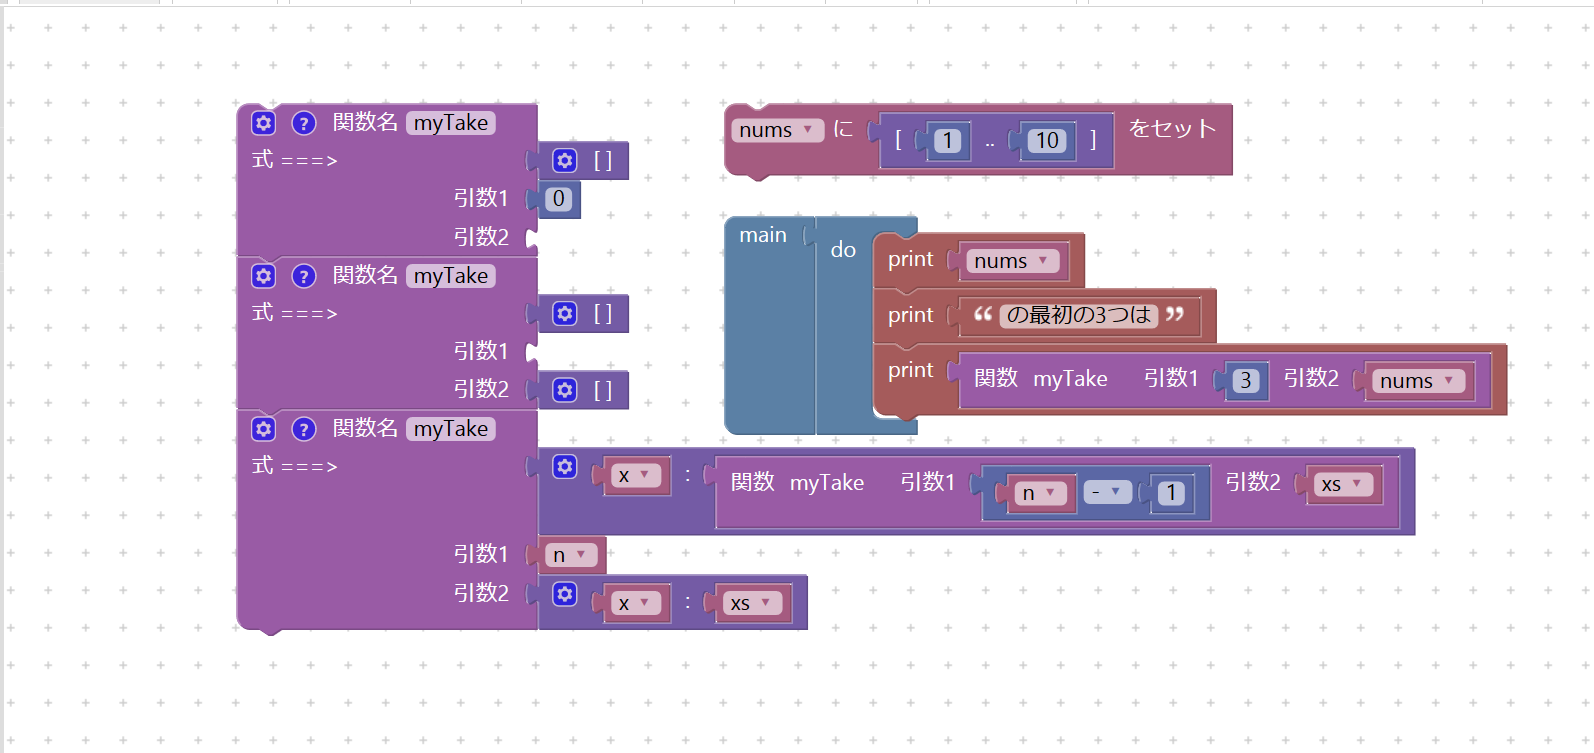
\includegraphics[scale=0.5]{img/haskell_experiment_result_a.PNG}
\caption{Aの完成されたHaskellコードのブロックは完成図}%
\label{fig:haskell_experiment_result_a}
\end{center}%
\end{figure}% 

Bの完成されたHaskellコードのブロックは図\ref{fig:haskell_experiment_result_b}に、そのHaskellのコードは以下である。merge関数は、2つのリストを昇順に重複無しで合成する関数である。
\begin{lstlisting}[basicstyle=\ttfamily\footnotesize]
merge [] ys = ys
merge xs [] = xs

merge (x:xs) (y:ys)
  | x == y = (x:merge xs ys)
  | x < y = (x:merge xs (y:ys))
  | x > y = (y:merge (x:xs) ys)
\end{lstlisting}

\begin{figure}[h]
\begin{center}
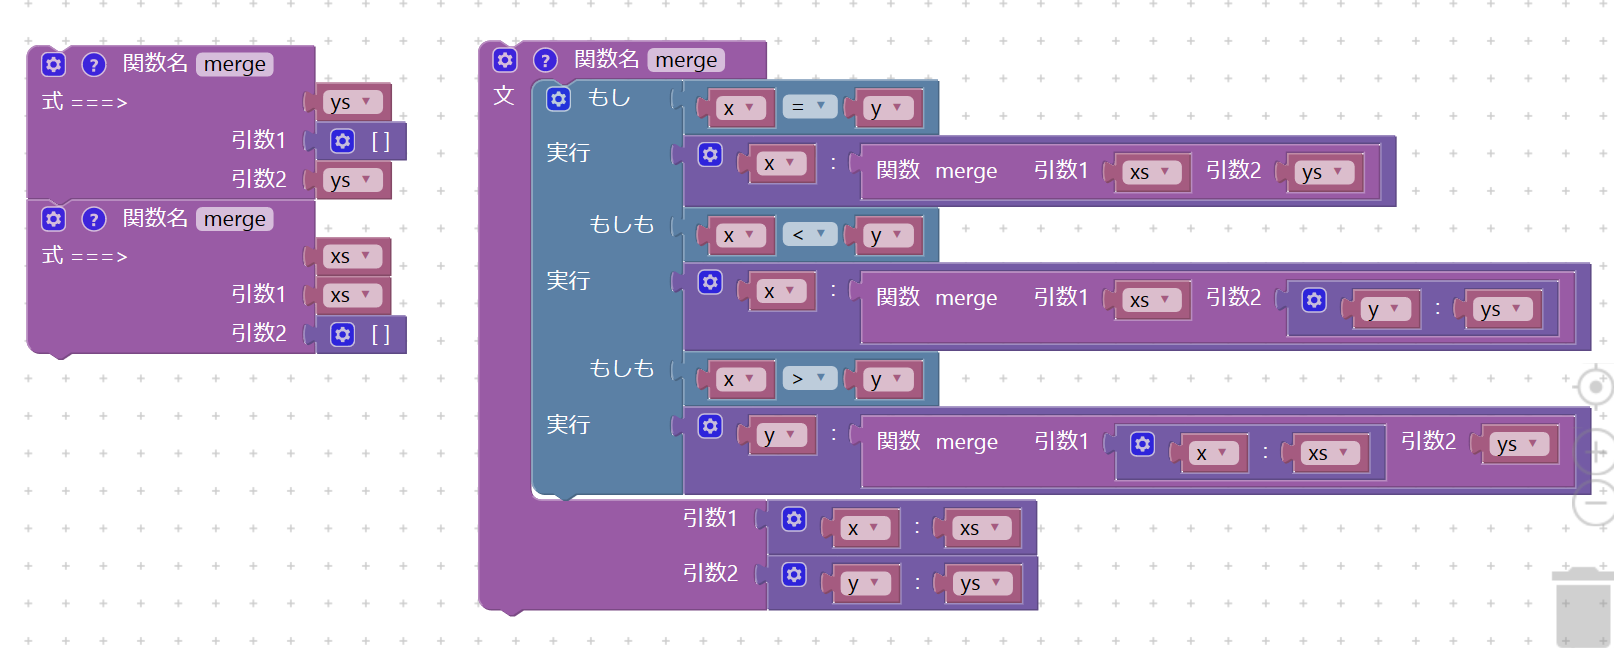
\includegraphics[scale=0.5]{img/haskell_experiment_result_b.PNG}
\caption{Bの完成されたHaskellコードのブロックは完成図}%
\label{fig:haskell_experiment_result_b}
\end{center}%
\end{figure}% 

\end{itemize} 

   		\subsection{改善した点}
        
Haskellの学習経験がほとんどない被験者3人に本研究のHaskellシステムを試してもらった。3人中2人が、Haskellの完成されたコードをブロックで組み立てることができたが、2時間から3時間と時間がかかっている状態であった。これらの要因としてシステムを理解するのに時間がかかっている状況であった。そこで、チュートリアルページの作成を行った。また、「関数の定義が見た目でわかりづらい」といった意見や「関数呼び出しブロックの生成が気づきにくい」といった意見があったので関数ブロックと関数呼び出しブロックを改善した。そして、「Web上で実行結果が表示できるようにして欲しい」という回答があったので、実行結果機能を実装した。各種機能の実装や改善したブロックの詳細な内容は、第3章に述べてある。

		\subsection{2回目の評価結果}

以下は、2回目の評価実験の結果を各評価項目で簡潔にまとめものである。

\begin{itemize}
\item Haskellの学習経験

2回目の評価実験で利用してもらった2人は、1回目の評価実験のときとは違う人物である。また、2人とも本研究のゼミで少しHaskellを学習した程度で初学者である。

\item Blockly for Haskell を使用した時間

1人は30分で、もう1人は1時間程度である。

\item 改善した方がいいと思うところ

- 実行結果というタブがありますが、どこから実行すればいいのか分からなかった

- 実行結果が表示できない場合、ブロックのどこが間違っているのかが分かると使いやすいと思った

- 作成したコードを保存して開こうとすると、インターネットエクスプローラーで勝手に開かれ、謎の文字列が表示される

\item 意見や感想

- 使いやすかった

- 使い方の説明書や、サンプルコードもあり非常に使いやすいアプリケーションだと思った

- コード化やブロックの保存もできる点が優れていると感じた

\item バグ報告 (非必須)

バグは報告されなかった。チュートリアルのページの間違いを1点指摘された。

\item 作成したブロックXMLコード

2人共、完成されたHaskellコードのブロックを組み立てることができた。2人の被験者の名称をそれぞれC, Dとする。

Cの完成されたHaskellコードのブロックは図\ref{fig:haskell_experiment_result_c}に、そのHaskellのコードは以下である。foo関数で内包表記が使われている。
\begin{lstlisting}[basicstyle=\ttfamily\footnotesize]
foo n = [ (x, y) |
    x <- [0..n]
  , y <- [x..n]
  ]
main = do
    putStr (foo 6)
\end{lstlisting}

\begin{figure}[h]
\begin{center}
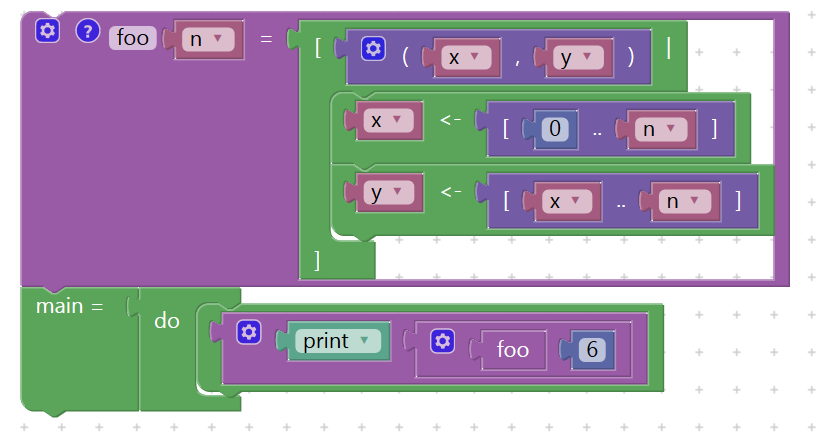
\includegraphics[scale=0.5]{img/haskell_experiment_result_c.PNG}
\caption{Cの完成されたHaskellコードのブロックは完成図}%
\label{fig:haskell_experiment_result_c}
\end{center}%
\end{figure}% 

Dの完成されたHaskellコードのブロックは図\ref{fig:haskell_experiment_result_d}に、そのHaskellのコードは以下である。fromBinAux関数は、初期値(第1引数)とbool型のリスト(第2引数)から末尾再帰で計算していく関数である。

\begin{lstlisting}[basicstyle=\ttfamily\footnotesize]
judge n = if n then 1 else 0
fromBinAux n [] = n
fromBinAux n (x:xs) = fromBinAux (n * 2 + judge x) xs
fromBin xs = fromBinAux 0 xs
main = do
    print (fromBin [True, False, True, False])
\end{lstlisting}

\begin{figure}[h]
\begin{center}
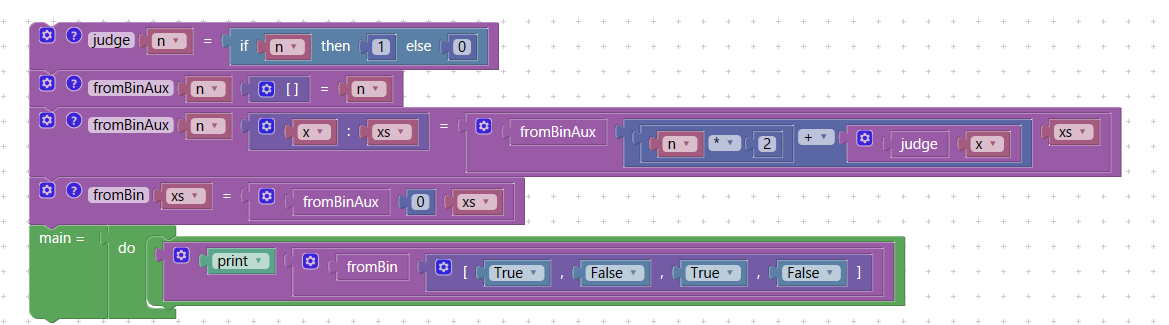
\includegraphics[scale=0.5]{img/haskell_experiment_result_d.PNG}
\caption{Dの完成されたHaskellコードのブロックは完成図}%
\label{fig:haskell_experiment_result_d}
\end{center}%
\end{figure}% 

\end{itemize} 

		\subsection{考察}
        
1回目の評価実験に比べて2回目の評価実験は、被験者のシステム利用時間が短縮された。これらの要因として、チュートリアルのページでブロックの組み立て方を掲載したのが要因であると考えられる。実際に、「使い方の説明書や、サンプルコードもあり非常に使いやすいアプリケーションだと思った」という意見を得ることができた。

2回目にの評価実験で新たに実装した実行結果機能では、「実行結果というタブがありますが、どこから実行すればいいのか分からなかった」という意見や「実行結果が表示できない場合、ブロックのどこが間違っているのかが分かると使いやすいと思った」という改善点を指摘された。実行結果機能については、使いづらかったようでさらなる改善が必要である。

   \section{Blockly for Flex の評価}
   
   		\subsection{評価方法}
        
本年度前期の「コンパイラデータベース演習」を履修している31名に評価してもらった。履修生が授業での演習問題に取り組んでいる際、もし行き詰ったりコードが理解できない場合に演習問題に平行してFlexシステムを自由に使用してもらった。そして、演習授業の終了後にアンケートに答えてもらい、以下の評価項目に4段階で回答する形式で行った。
\begin{itemize}
\item Q1. あなたはプログラミングが得意ですか?
\item Q2. コンパイラデータベース演習を通してFlex(字句解析)は理解できましたか?
\item Q3. 演習中にBlockly for Flexをどの程度利用しましたか?
\item Q4. Blockly for Flex が今回の演習に役に立ちましたか?
\item Q5. Blockly for Flex のシステムについて理解しやすかったですか?
\item Q6. システム全体の評価
\end{itemize} 
評価段階は、Q1, Q2, Q4, Q5の場合は、そう思う、どちらかといえばそう思う、どちらかといえばそう思わない、そう思わないの4段階で、Q5の場合は、とても利用した、まあまあ利用した、少し利用した、全く利用しなかったの4段階である。
さらに最後の評価項目にシステムの全体評価をとても良い・良い・普通・悪い・とても悪いの5段階でやってもらい、理由を書ける自由記述の欄も設けた。評価アンケートは匿名性で、アンケート用紙を配布しオフライン形式で行った。

オフライン形式で行った理由は、アンケート用紙だとその場で提出しなければならないが、オンライン形式だと時間、場所を問わずに提出できるので提出を後回しにされてしまい最終的に出し忘れるの場合があるのでそれを防ぐためである。以下の図\ref{fig:questionnaire}は、実際のアンケート用紙である。

\begin{figure}[h]
\begin{center}
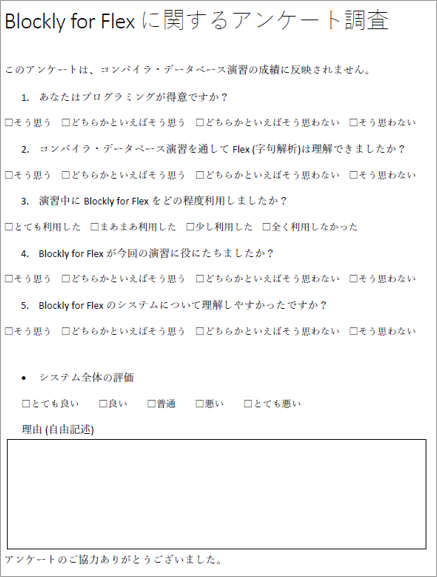
\includegraphics[scale=1.0]{img/questionnaire.PNG}
\caption{実際のアンケート用紙}%
\label{fig:questionnaire}
\end{center}%
\end{figure}% 


   		\subsection{評価結果}

アンケート結果をそれぞれの質問に対する回答結果を棒グラフ化したものを以下の図\ref{fig:flex_bar_graph}に示す。そして、その棒グラフの凡例は、図\ref{fing:flex_usage_guide}で、左はQ1, Q2, Q4, Q5の凡例で、真ん中はQ3の凡例で、右はQ6の凡例である。

\begin{figure}[h]
\begin{center}
\includegraphics[scale=1.0]{img/flex_bar_graph.PNG}
\caption{それぞれの質問に対する回答結果}%
\label{fig:flex_bar_graph}
\end{center}%
\end{figure}% 

\begin{figure}[h]
\begin{center}
\includegraphics[scale=1.0]{img/flex_usage_guide.PNG}
\caption{評価段階の凡例}%
\label{fing:flex_usage_guide}
\end{center}%
\end{figure}% 

   		\subsection{システム全体の評価理由}

理由を書ける自由記述の欄で、システム全体の評価とその理由を書いてもらった。以下は、具体的なシステム全体の評価とその理由である。「利用できなかった」という回答が7件あった。

\begin{itemize}
\item システム全体の評価:良い

- 実際に使用しなかったため、はっきりとは言えないが、見ただけである程度どう使えばいいのか分かったように思うため。

- Flexの予備知識が十分にないと上手に使いこなせないと思う。演習の問題で試してみたがエラーが出て、自分でプログラムを組んでいないため、どこがだめなのか分かりづらかった。

- 提出時間のことを考えて、使うことはなかったけど、話を聞いて役に立つものだと思いました。

\item システム全体の評価:普通

- ブロック→ コード にしたいと思う機会がない。せめて出力機能をつけてほしい。

- 今回の演習は、資料等を見たり、人に聞くことで解くことができたため、使おうと思う場面がありませんでした。

\item システム全体の評価:悪い

- 初めて使う際に、分かりづらい。どのようにプログラムを書くか等。

\item システム全体の評価:未回答

- 時間がなかったので利用できませんでした。

- 理解するのでいっぱいで使えませんでした。

\end{itemize} 

        \subsection{考察}

まず、「コンパイラデータベース演習」を履修している31名は、Flexを初めて学習する人がほとんどで本システムの対象者であるプログラミング初学者と一致している。


Q1の「あなたはプログラミングが得意ですか?」では、どちらかといえばそうではない・そうではないという回答が過半数を占め、履修生の傾向としてプログラミングが得意ではないという人が多いという結果であった。そのなかでもQ2の結果から今回のコンパイラデータベース演習ではそう思う・どちらかといえばそう思うが過半数を占め、Flexの内容を理解できた状況であった。Q3の「演習中にBlockly for Flexをどの程度利用しましたか?」では、約4分の3はほとんど利用していないという結果であった。この結果から、問4から問6にある一定数の未回者がいる原因となっている。システムの使い方の理解度やシステム全体の評価は、過半数の人が肯定的な評価を示している。
   \section{Blockly for Prolog の評価}
   
		\subsection{評価方法}

2020年1月に香川研究室の学部生2名を対象に行った。被験者は、2回目のHaskellの評価実験と同じ被験者でHaskellのシステムを利用してもらった後にPrologのシステムページにアクセスしてもらい、チュートリアルのページでブロックの組み立て方を見ながらシステムを利用してもらう。そして、以下の評価項目に自由に回答する形式で行った。

\begin{itemize}
\item prolog の学習経験
\item Blockly for Prolog を使用した時間
\item 改善した方がいいと思うところ
\item 意見や感想
\item バグ報告 (非必須)
\item 作成したブロックXMLコード
\end{itemize} 

		\subsection{評価結果}

以下は、評価実験の結果を各評価項目で簡潔にまとめものである。

\begin{itemize}
\item Prologの学習経験

2人とも、Prologに触れるのが初めてで初学者である。Blocklyを通して初めてprologのプログラムを組み立てることになる。

\item Blockly for Prolog を使用した時間

2人とも、30分程度利用した。

\item 改善した方がいいと思うところ

- ブロックを同じカテゴリから複数持ってきたいときに、カテゴリが閉じてしまい、少し不便だったため複数選択やカテゴリを閉じないようにする
ことができたらいいなと思った

- アプリケーションに関してはHaskellと同様である

\item 意見や感想

- 視覚的に理解することができ、知らない言語でもある程度理解することができた

- ネットでもPrologの情報が少なく、初修者に関しては難しいアプリケーションであると感じた

- UIに関しては使いやすいものである思う

- 保存や読込などもユーザが直観的な操作が可能であると感じた

\item バグ報告 (非必須)

サンプル機能に関してバグが1点を報告された。詳細な内容は割愛する。

\item 作成したブロックXMLコード

2人とも完成されたPrologコードのブロックを組み立てることができた。2人の被験者の名称をそれぞれA, Bとする。

Aの完成されたPrologコードのブロックは図\ref{fig:prolog_experiment_result_a}に、そのPrologのコードは以下である。
\begin{lstlisting}[basicstyle=\ttfamily\footnotesize]
myAppend([],Y,Y) :-
    myAppend([H|X],Y,[H|Z]).

myAppend(X,Y,Z).

?- myAppend(X,Y,[1,2,3]).
\end{lstlisting}

\begin{figure}[h]
\begin{center}
\includegraphics[scale=0.5]{img/prolog_experiment_result_a.PNG}
\caption{Aの完成されたPrologコードのブロックは完成図}%
\label{fig:prolog_experiment_result_a}
\end{center}%
\end{figure}% 

Bの完成されたPrologコードのブロックは図\ref{fig:prolog_experiment_result_b}に、そのPrologのコードは以下である。
\begin{lstlisting}[basicstyle=\ttfamily\footnotesize]
father(ieyasu,hirotada).

father(hirotada,kiyoyasu).

granpa(GC,GP) :-
    father(GC,C),
    father(C,GP).

?- granpa(ieyasu,X).
\end{lstlisting}

\begin{figure}[h]
\begin{center}
\includegraphics[scale=0.5]{img/prolog_experiment_result_b.PNG}
\caption{Bの完成されたPrologコードのブロックは完成図}%
\label{fig:prolog_experiment_result_b}
\end{center}%
\end{figure}% 

\end{itemize} 
        
		\subsection{考察}
        
Haskellの評価実験後にPrologの評価実験を行ったので、システムの理解については問題なく30分という短い時間で完成されたブロックを組み立てることができていた。しかし、2人ともPrologに関しては、全くの初学者であったので、完成されたブロックのPrologのソースコードはシンプルであった。文法の基礎は理解してもらえた様子である。

   \chapter{おわりに}
   
   \section{まとめ}
   
本研究では、大学の講義で学習するプログラミング言語に対応させるために、Blocklyの多言語化を行った。対応言語は、C、JavaScript、Haskell、Bison Flex、Prolog、Scheme、Pythonである。それぞれの言語システムでプログラミング言語に対応した文法に対応した新たなブロックをいくつか実装した。その際、プログラミング言語の柔軟性を保持するために、ブロックの動的変形機能の拡張も行った。

2回目のHaskellシステムの評価実験で得られたフィードバックを通して、実装したブロックを改善し、チュートリアルのページを作成した。また、被験者の要望により実行機能も実装した。しかし、新たに実装した実行結果機能について使いづらいといったフィードバックを得られたので改善が必要である。

Flexシステムの評価実験では、演習時間内という限られた時間内での評価実験であったため、一定数の利用できなかった被験者がいたものの利用してくれた被験者からは、過半数の人が肯定的な評価を示した。

Prologシステムの評価実験でも被験者はBlocklyを通して文法の理解をしてもらえた。

これらの評価実験の結果から、いくつかの課題点はあるものの本研究で実装したシステムは第1章でのシステムに求められる要件を満たしたと言える。

   \section{今後の課題}
   
以下に本システムの今後の課題を述べる。
   
\begin{itemize}

\item 実行結果機能の改善

2回目のHaskellの評価実験において、「実行結果というタブがありますが、どこから実行すればいいのか分からなかった」、「実行結果が表示できない場合、ブロックのどこが間違っているのかが分かると使いやすいと思った」といった意見が得られた。これらのフィードバックをもとに、実行結果機能のUIの改善と実行結果が表示されない場合のエラー表示とエラーの原因がどこのコードの部分かをBlocklyのブロックで可視化する必要がある。

\item Flexシステムの簡素化

Flexシステムの評価実験において、ある一定数の被験者が時間の都合上利用できなかった。時間があまりない状況では、手軽に使えるシステムを目指さなければなたない。そこで、Flexの重要部分である動作の正規表現を分かりやすく扱えるようにFlexシステムの簡素化する必要がある。具体案としては、制御ブロックや関数ブロックを消去するなどである。

\item ソースコードからのブロック生成機能の拡張

関連研究である山形のシステムでは、C言語ソースコ-ドからXMLへ変換してブロックを生成するといった機能がある。本システムでは、Blockly C and Python に一部実装してある。しかし、C言語のソースコードからブロックを生成できてもPythonのソースコードからブロックを生成することができない。そこで、まずはPythonのソースコードからブロックを生成できることを目指して、そこから他の言語システムでもソースコードからブロックを生成できるように機能を拡張していく必要がある。

\end{itemize} 
 

\acknowledgment  % 謝辞

本研究においてご指導を受け賜りました香川考司先生と協力してくださった香川研究室の皆様に心からの感謝の意を表します。また、本年度前期の「コンパイラデータベース演習」の履修生の方々に評価実験に協力していただきました。ありがとうございました。そして、副査として厳正なる審査をいただいた最所先生、高木先生に心より厚くお礼申し上げます。

\begin{thebibliography}{99} % 参考文献
                                  
  \bibitem{Blockly} % 論文
 Google 
 ``Blockly'', https://developers.google.com/blockly/, 2020年2月閲覧.

  \bibitem{Scratch} % 論文
 MITメディアラボ, Lifelong Kindergarten Group 
 ``Scratch'', https://developers.google.com/blockly/, 2020年2月閲覧.
 
  \bibitem{waterbear} % 論文
 Dethe Elza
 ``waterbear'', https://waterbearlang.com/, 2020年2月閲覧.

  \bibitem{ozaki} % 論文
 尾崎陽一,
 ``Webベースグラフィカルプログラミングエディタを用いた円滑な移行が可能なC言語学習支援環境の開発'', 香川大学大学院工学研究科信頼性情報システム工学専攻 2014年度修士論文, 2015年.
 
  \bibitem{yamagata} % 論文
 山形悠人
 ``Blockly プログラム生成の自動化によるWebベースC言語学習支援環境の機能拡張'', 香川大学大学院工学研究科
博士前期課程信頼性情報システム工学専攻2017年度修士論文, 2018年.

  \bibitem{yamagata2} % 論文
 Yuto Yamagata and Koji Kagawa
 ``A Web-based Learning Support System for the C Language with Automatic Generation of Blockly Programs'', EdMedia + Innovate Learning 2018, Amsterdam, Netherlands, June 2018
 
  \bibitem{otya} % 論文
 松本晴香, 浅井健一
 ``Blockly をベースにしたOCamlビジュアルプログラミングエディタ'', PPL2019, 第21回プログラミングおよびプログラミング言語ワークショップ論文集 15ページ.
 
  \bibitem{idc} % 論文
 David Weintrop, Uri Wilensky
 ``To Block or not to Block, That is the Question: Students’ Perceptions of Blocks-based Programming
'', IDC'15, June 2015. 

  \bibitem{flex} % 論文
 G. T. Nicol
 ``Flex: the lexical scanner generator, Free Software Foundation'', 1993.
 
  \bibitem{prolog} % 論文
 Nitta Lab., Computer Science, Tsuda University, Japan.
 ``Prolog'', https://nw.tsuda.ac.jp/lec/prolog/, 2020年2月閲覧.

\end{thebibliography}



\insertindex % 索引を出力                                 
\printindex
  
\end{document}
